\documentclass[]{report}
\usepackage{lmodern}
\usepackage{setspace}
\setstretch{1}
\usepackage{amssymb,amsmath}
\usepackage{ifxetex,ifluatex}
\usepackage{fixltx2e} % provides \textsubscript
\ifnum 0\ifxetex 1\fi\ifluatex 1\fi=0 % if pdftex
  \usepackage[T1]{fontenc}
  \usepackage[utf8]{inputenc}
\else % if luatex or xelatex
  \ifxetex
    \usepackage{mathspec}
  \else
    \usepackage{fontspec}
  \fi
  \defaultfontfeatures{Ligatures=TeX,Scale=MatchLowercase}
\fi
% use upquote if available, for straight quotes in verbatim environments
\IfFileExists{upquote.sty}{\usepackage{upquote}}{}
% use microtype if available
\IfFileExists{microtype.sty}{%
\usepackage{microtype}
\UseMicrotypeSet[protrusion]{basicmath} % disable protrusion for tt fonts
}{}
\usepackage[margin=1in]{geometry}
\usepackage{hyperref}
\hypersetup{unicode=true,
            pdftitle={How to create and edit maps with R},
            pdfauthor={Kévin Cazelles},
            pdfborder={0 0 0},
            breaklinks=true}
\urlstyle{same}  % don't use monospace font for urls
\usepackage{color}
\usepackage{fancyvrb}
\newcommand{\VerbBar}{|}
\newcommand{\VERB}{\Verb[commandchars=\\\{\}]}
\DefineVerbatimEnvironment{Highlighting}{Verbatim}{commandchars=\\\{\}}
% Add ',fontsize=\small' for more characters per line
\usepackage{framed}
\definecolor{shadecolor}{RGB}{248,248,248}
\newenvironment{Shaded}{\begin{snugshade}}{\end{snugshade}}
\newcommand{\KeywordTok}[1]{\textcolor[rgb]{0.13,0.29,0.53}{\textbf{{#1}}}}
\newcommand{\DataTypeTok}[1]{\textcolor[rgb]{0.13,0.29,0.53}{{#1}}}
\newcommand{\DecValTok}[1]{\textcolor[rgb]{0.00,0.00,0.81}{{#1}}}
\newcommand{\BaseNTok}[1]{\textcolor[rgb]{0.00,0.00,0.81}{{#1}}}
\newcommand{\FloatTok}[1]{\textcolor[rgb]{0.00,0.00,0.81}{{#1}}}
\newcommand{\ConstantTok}[1]{\textcolor[rgb]{0.00,0.00,0.00}{{#1}}}
\newcommand{\CharTok}[1]{\textcolor[rgb]{0.31,0.60,0.02}{{#1}}}
\newcommand{\SpecialCharTok}[1]{\textcolor[rgb]{0.00,0.00,0.00}{{#1}}}
\newcommand{\StringTok}[1]{\textcolor[rgb]{0.31,0.60,0.02}{{#1}}}
\newcommand{\VerbatimStringTok}[1]{\textcolor[rgb]{0.31,0.60,0.02}{{#1}}}
\newcommand{\SpecialStringTok}[1]{\textcolor[rgb]{0.31,0.60,0.02}{{#1}}}
\newcommand{\ImportTok}[1]{{#1}}
\newcommand{\CommentTok}[1]{\textcolor[rgb]{0.56,0.35,0.01}{\textit{{#1}}}}
\newcommand{\DocumentationTok}[1]{\textcolor[rgb]{0.56,0.35,0.01}{\textbf{\textit{{#1}}}}}
\newcommand{\AnnotationTok}[1]{\textcolor[rgb]{0.56,0.35,0.01}{\textbf{\textit{{#1}}}}}
\newcommand{\CommentVarTok}[1]{\textcolor[rgb]{0.56,0.35,0.01}{\textbf{\textit{{#1}}}}}
\newcommand{\OtherTok}[1]{\textcolor[rgb]{0.56,0.35,0.01}{{#1}}}
\newcommand{\FunctionTok}[1]{\textcolor[rgb]{0.00,0.00,0.00}{{#1}}}
\newcommand{\VariableTok}[1]{\textcolor[rgb]{0.00,0.00,0.00}{{#1}}}
\newcommand{\ControlFlowTok}[1]{\textcolor[rgb]{0.13,0.29,0.53}{\textbf{{#1}}}}
\newcommand{\OperatorTok}[1]{\textcolor[rgb]{0.81,0.36,0.00}{\textbf{{#1}}}}
\newcommand{\BuiltInTok}[1]{{#1}}
\newcommand{\ExtensionTok}[1]{{#1}}
\newcommand{\PreprocessorTok}[1]{\textcolor[rgb]{0.56,0.35,0.01}{\textit{{#1}}}}
\newcommand{\AttributeTok}[1]{\textcolor[rgb]{0.77,0.63,0.00}{{#1}}}
\newcommand{\RegionMarkerTok}[1]{{#1}}
\newcommand{\InformationTok}[1]{\textcolor[rgb]{0.56,0.35,0.01}{\textbf{\textit{{#1}}}}}
\newcommand{\WarningTok}[1]{\textcolor[rgb]{0.56,0.35,0.01}{\textbf{\textit{{#1}}}}}
\newcommand{\AlertTok}[1]{\textcolor[rgb]{0.94,0.16,0.16}{{#1}}}
\newcommand{\ErrorTok}[1]{\textcolor[rgb]{0.64,0.00,0.00}{\textbf{{#1}}}}
\newcommand{\NormalTok}[1]{{#1}}
\usepackage{longtable,booktabs}
\usepackage{graphicx,grffile}
\makeatletter
\def\maxwidth{\ifdim\Gin@nat@width>\linewidth\linewidth\else\Gin@nat@width\fi}
\def\maxheight{\ifdim\Gin@nat@height>\textheight\textheight\else\Gin@nat@height\fi}
\makeatother
% Scale images if necessary, so that they will not overflow the page
% margins by default, and it is still possible to overwrite the defaults
% using explicit options in \includegraphics[width, height, ...]{}
\setkeys{Gin}{width=\maxwidth,height=\maxheight,keepaspectratio}
\IfFileExists{parskip.sty}{%
\usepackage{parskip}
}{% else
\setlength{\parindent}{0pt}
\setlength{\parskip}{6pt plus 2pt minus 1pt}
}
\setlength{\emergencystretch}{3em}  % prevent overfull lines
\providecommand{\tightlist}{%
  \setlength{\itemsep}{0pt}\setlength{\parskip}{0pt}}
\setcounter{secnumdepth}{5}
% Redefines (sub)paragraphs to behave more like sections
\ifx\paragraph\undefined\else
\let\oldparagraph\paragraph
\renewcommand{\paragraph}[1]{\oldparagraph{#1}\mbox{}}
\fi
\ifx\subparagraph\undefined\else
\let\oldsubparagraph\subparagraph
\renewcommand{\subparagraph}[1]{\oldsubparagraph{#1}\mbox{}}
\fi

%%% Use protect on footnotes to avoid problems with footnotes in titles
\let\rmarkdownfootnote\footnote%
\def\footnote{\protect\rmarkdownfootnote}

%%% Change title format to be more compact
\usepackage{titling}

% Create subtitle command for use in maketitle
\newcommand{\subtitle}[1]{
  \posttitle{
    \begin{center}\large#1\end{center}
    }
}

\setlength{\droptitle}{-2em}
  \title{How to create and edit maps with R}
  \pretitle{\vspace{\droptitle}\centering\huge}
  \posttitle{\par}
  \author{Kévin Cazelles}
  \preauthor{\centering\large\emph}
  \postauthor{\par}
  \predate{\centering\large\emph}
  \postdate{\par}
  \date{March 31, 2015}

\usepackage{fancyhdr}
\pagestyle{fancy}
\fancyhead[CO,CE]{}
\fancyfoot[CO,CE]{Making maps with R}
\fancyfoot[LE,RO]{\thepage}

\begin{document}
\maketitle
\begin{abstract}
This manuals is dedicated to readers who wants to get started with map
creation and edition in R. It provides a basic understanding of the
fundamental packages and functions required to turn R into an efficient
Geographic Information System (GIS). It also shows how to manipulated
the spatial objects defined. It is however beyond the range of this
document to present exhaustively the potentialities R offers in term of
spatial manipulations and analyses. Rather, it focuses on explaining
what are the essential classes of spatial objects and the methods that
can be applied and pinpoints valuable resources for readers who want to
go further.
\end{abstract}


Ce document est distribu\'{e} sous les termes de la licence CC-BY-NC-SA 4.0, licence de libre diffusion soumise à certaines conditions. En accord avec cette licence, vous pouvez librement utiliser, adapter, modifier et redistribuer le contenu de ce document dans n'importe quelle circonstance, sauf à des fins commerciales (NC), et à la condition non-n\'{e}gociable qu’un cr\'{e}dit suffisant soit attribu\'{e} à l'auteur de ce pr\'{e}sent document en citant leurs noms (BY). Toute version modifi\'{e}e et redistribu\'{e}e sera r\'{e}gie par les m\^{e}mes termes (SA). Ces droits et conditions seront valides tant que le pr\'{e}sent travail sera plac\'{e} sous les termes de cette licence.

\begin{center}

\includegraphics[width=.28\textwidth]{aux/ccbyncsa.png}
\end{center}


\newpage

{
\setcounter{tocdepth}{2}
\tableofcontents
}
\listoffigures
\chapter{Introduction}\label{introduction}

Since the last decade, new softwares have emerged making the creation
and edition of maps accessible to all. Scientists can now readily draw
valuable spatial representations of their work without deep knowledge in
mapping\footnote{I recommend the reading of the article:
  \href{http://www.nature.com/news/data-visualization-science-on-the-map-1.17024}{Zastrow,
  Mark. 2015. ``Science on the Map.'' Nature 519: 119--120.}}. Basic
mapping skills should be a part of educational background of most of
scientists as maps are often a proper way to expose facts and thereby
relevant representations that may ease the scientific debate. Among the
tools available (see below) some Geographic Information System (GIS) are
free, open-source such as \href{http://qgis.org/en/site/}{Quantum GIS}
and \href{http://grass.osgeo.org}{GRASS GIS}. Also, some high-level
programming languages such as JavaScript, Python, or R offer dedicated
packages. Few software are listed a couple of softwares:

\begin{itemize}
\tightlist
\item
  \href{http://www.arcgis.com/features/}{ArcGIS}
\item
  \href{http://cartodb.com}{CartoDB}
\item
  \href{http://www.diva-gis.org}{DIVA-GIS}
\item
  \href{http://geojson.io/\#map=2/20.0/0.0}{GeoJson}
\item
  \href{https://www.google.fr/maps}{Google Map}
\item
  \href{http://www.google.fr/intl/eng/earth/index.html}{Goole Earth}
\item
  \href{http://grass.osgeo.org}{GRASS}
\item
  \href{http://leafletjs.com}{Leaflet}
\item
  \href{http://www.mapinfo.com}{Mapinfo}
\item
  \href{http://mapnik.org}{Mapnik}
\item
  \href{http://www.postgis.org}{PostGIS}
\item
  \href{http://qgis.org/en/site/}{Quantum GIS}
\item
  \href{http://www.saga-gis.org/en/index.html}{SAGA GIS}
\item
  \href{https://www.mapbox.com/tilemill/}{TileMill}
\end{itemize}

\section{Why use R for mapping?}\label{why-use-r-for-mapping}

Given the number of tools dedicated to visualization and analyses of
spatial data, it is important that users ask this question and take some
time and balance pros ans cons. According to me, the choice strongly
relies upon (i) your ambition in term of mapping and (ii) your R skills.
If you aim at creating a good-looking map without analysis and you are
not familiar with R, I would discourage you to use R. But if you are
familiar with R, you can quickly get a map as a R plot and so benefit
from the plot system you already know. Also, when you need tricky
spatial analysis (\emph{e.g} krigging), even if you are not familiar
with R, you may benefit from this language and you may not encounter any
difficulties to realize any kind of analysis and gather the plot.
Ultimately yo will analysis and create your plot with R only.

\section{What can be found in this
document?}\label{what-can-be-found-in-this-document}

This short document provides some basics to create and edit maps using
\href{https://cran.r-project.org}{R}. One of the strongest advantage of
using R as a Geographic Information System (GIS) is to use its
facilities to manipulate efficiently spatial object and to undertake
various spatial analysis. The spatial analysis are beyond the scope of
this document. I will deal with the manipulation of spatial objects: I
start by explaining how spatial classes work in R, then I show you how R
can import and export spatial objects. The latter makes R a useful tool
to create, manipulate and convert files that contain spatial data.
Throughout the document I strive to provide advices (as good as
possible) to edit simple but elegant maps.

To be able to use all the code below, four packages must be installed:
``sp'', ``raster'', ``rgdal'', ``rgeos''. Their installation will be
explained along the document. To take maximum benefits from the present
document you must be working on line. As the reader of this document,
you must have basic R skills, meaning the user knows how to use object,
how to code basic functions and how to edit plots. If it not the case,
you may benefit from a clear introduction to R such as the one available
on the
\href{http://cran.r-project.org/doc/manuals/r-release/R-intro.html}{CRAN
website}.

If the reader of the present document is eager to learn more about the
potentialities R offers, a good starting point is to read the valuable
\href{http://cran.r-project.org/web/views/Spatial.html}{package guide}
Roger Bivand - one of the most important contributor to spatial analysis
in R - wrote. You can also pursue your learning by having a look of the
\href{http://link.springer.com/book/10.1007/978-1-4614-7618-4}{book} the
same author wrote with two colleagues.

\section{Colophon}\label{colophon}

The present document has been written using
\href{http://rmarkdown.rstudio.com/authoring_rcodechunks.html}{R
Markdown} on MacOSX 10.10.4. I conceived the code to make it working
standalone: additional material is downloaded from R commands. Also,
instead of a reference list, I provide hyper-links to better explain
what we do when we use spatial object in R. The version of R that
creates the document is:

As a convention, I use bold fonts for R objects and I add parentheses
for objects that are functions (\emph{e.g.}, object \textbf{obj} and
function \textbf{foo()}). I use italics for class and function arguments
(for instance, argument \emph{arg}) and I employ quotemarks for package
names (\emph{e.g}, package ``sp''). Also, \emph{path} denotes the
character string that contains the path of the ``.Rmd'' file that
generates this document. If you find some error or have any comments
about this document and/or the script, please feel free to send me an
email (kevin(dot)cazelles(at)gmail(dot)com).

Many functions are used throughout this document and some are not
detailed. Whenever you want to get more details, I recommend you to read
the documentation associated. To get access to this documentation, you
need to type ``?'' before the name of the function then press Enter in
the R console. The example below shows two commands to access the help
associated to the \textbf{getwd()} function.

\begin{Shaded}
\begin{Highlighting}[]
\NormalTok{?getwd}
\KeywordTok{help}\NormalTok{(}\StringTok{"getwd"}\NormalTok{)}
\end{Highlighting}
\end{Shaded}

\chapter{Points, Lines, Polygons and
Grids}\label{points-lines-polygons-and-grids}

Basically, spatial objects are split into two categories: vectors and
rasters. Roughly speaking, vectors are a set of coordinates, whereas
rasters are regular grids. The first step to create a map is to
manipulate points, lines and grids (polygons can be considered as a sets
of closed lines). This is what I present in this section. At first
glance, one can describe our planet as a sphere and locate any point on
Earth by two values: the longitude (values taken in {[}-180,180{]}) and
the latitude (values taken in {[}-90,90{]})\footnote{Obviously, there
  are many ways to locate points on Earth.}. For the sake of
illustration, I define a object \textbf{vec} that contains the
coordinates of 10 points randomly distributed on Earth .

\begin{Shaded}
\begin{Highlighting}[]
\NormalTok{nbp <-}\StringTok{ }\DecValTok{10}
\NormalTok{vec <-}\StringTok{ }\KeywordTok{list}\NormalTok{(}\DataTypeTok{x=}\KeywordTok{runif}\NormalTok{(nbp,-}\DecValTok{160}\NormalTok{,}\DecValTok{160}\NormalTok{), }\DataTypeTok{y=}\KeywordTok{runif}\NormalTok{(nbp,-}\DecValTok{80}\NormalTok{,}\DecValTok{80}\NormalTok{))}
\end{Highlighting}
\end{Shaded}

\begin{Shaded}
\begin{Highlighting}[]
\NormalTok{ras <-}\StringTok{ }\KeywordTok{matrix}\NormalTok{(}\KeywordTok{runif}\NormalTok{(nbp*nbp),nbp)}
\end{Highlighting}
\end{Shaded}

To keep things as simple as possible, that is all that should be
defined! Drawing very basic maps is no more that plotting these objects:

\begin{Shaded}
\begin{Highlighting}[]
\CommentTok{# Split the plot region into four subregions, the box is of "L" form.}
\KeywordTok{par}\NormalTok{(}\DataTypeTok{mfrow=}\KeywordTok{c}\NormalTok{(}\DecValTok{2}\NormalTok{,}\DecValTok{2}\NormalTok{), }\DataTypeTok{bty=}\StringTok{"l"}\NormalTok{)}
\NormalTok{## ----}
\KeywordTok{plot}\NormalTok{(}\KeywordTok{c}\NormalTok{(-}\DecValTok{180}\NormalTok{,+}\DecValTok{180}\NormalTok{),}\KeywordTok{c}\NormalTok{(-}\DecValTok{90}\NormalTok{,}\DecValTok{90}\NormalTok{), }\DataTypeTok{col=}\DecValTok{0}\NormalTok{, }\DataTypeTok{main=}\StringTok{"Points"}\NormalTok{, }\DataTypeTok{xlab=}\StringTok{""}\NormalTok{, }\DataTypeTok{ylab=}\StringTok{"Latitude (°)"}\NormalTok{)}
\KeywordTok{points}\NormalTok{(vec, }\DataTypeTok{pch=}\DecValTok{19}\NormalTok{, }\DataTypeTok{col=}\KeywordTok{c}\NormalTok{(}\DecValTok{1}\NormalTok{,}\StringTok{"grey45"}\NormalTok{))}
\KeywordTok{text}\NormalTok{(vec$x, vec$y, }\DecValTok{1}\NormalTok{:}\DecValTok{10}\NormalTok{, }\DataTypeTok{pos=}\DecValTok{3}\NormalTok{, }\DataTypeTok{col=}\KeywordTok{c}\NormalTok{(}\DecValTok{1}\NormalTok{,}\StringTok{"grey45"}\NormalTok{))}
\NormalTok{## ----}
\KeywordTok{plot}\NormalTok{(}\KeywordTok{c}\NormalTok{(-}\DecValTok{180}\NormalTok{,+}\DecValTok{180}\NormalTok{),}\KeywordTok{c}\NormalTok{(-}\DecValTok{90}\NormalTok{,}\DecValTok{90}\NormalTok{), }\DataTypeTok{col=}\DecValTok{0}\NormalTok{, }\DataTypeTok{main=}\StringTok{"Lines"}\NormalTok{, }\DataTypeTok{xlab=}\StringTok{""}\NormalTok{, }\DataTypeTok{ylab=}\StringTok{""}\NormalTok{)}
\KeywordTok{lines}\NormalTok{(vec$x[}\DecValTok{1}\NormalTok{:}\DecValTok{4}\NormalTok{], vec$y[}\DecValTok{1}\NormalTok{:}\DecValTok{4}\NormalTok{])}
\KeywordTok{lines}\NormalTok{(vec$x[}\DecValTok{5}\NormalTok{:}\DecValTok{6}\NormalTok{], vec$y[}\DecValTok{5}\NormalTok{:}\DecValTok{6}\NormalTok{], }\DataTypeTok{col=}\DecValTok{2}\NormalTok{)}
\KeywordTok{lines}\NormalTok{(vec$x[}\DecValTok{7}\NormalTok{:}\DecValTok{10}\NormalTok{], vec$y[}\DecValTok{7}\NormalTok{:}\DecValTok{10}\NormalTok{], }\DataTypeTok{col=}\DecValTok{3}\NormalTok{)}
\NormalTok{## ----}
\KeywordTok{plot}\NormalTok{(}\KeywordTok{c}\NormalTok{(-}\DecValTok{180}\NormalTok{,+}\DecValTok{180}\NormalTok{),}\KeywordTok{c}\NormalTok{(-}\DecValTok{90}\NormalTok{,}\DecValTok{90}\NormalTok{), }\DataTypeTok{col=}\DecValTok{0}\NormalTok{, }\DataTypeTok{main=}\StringTok{"Polygon"}\NormalTok{, }\DataTypeTok{xlab=}\StringTok{"Longitude (°)"}\NormalTok{,}
    \DataTypeTok{ylab=}\StringTok{"Latitude (°)"}\NormalTok{)}
\KeywordTok{polygon}\NormalTok{(vec$x[}\DecValTok{1}\NormalTok{:}\DecValTok{6}\NormalTok{], vec$y[}\DecValTok{1}\NormalTok{:}\DecValTok{6}\NormalTok{], }\DataTypeTok{col=}\DecValTok{2}\NormalTok{, }\DataTypeTok{lwd=}\DecValTok{4}\NormalTok{, }\DataTypeTok{border=}\DecValTok{4}\NormalTok{)}
\NormalTok{## ----}
\KeywordTok{image}\NormalTok{(}\KeywordTok{seq}\NormalTok{(-}\DecValTok{120}\NormalTok{,}\DecValTok{120}\NormalTok{,}\DataTypeTok{length.out=}\DecValTok{11}\NormalTok{), }\KeywordTok{seq}\NormalTok{(-}\DecValTok{60}\NormalTok{,}\DecValTok{60}\NormalTok{,}\DataTypeTok{length.out=}\DecValTok{11}\NormalTok{), ras, }\DataTypeTok{main=}\StringTok{"Grid"}\NormalTok{,}
    \DataTypeTok{xlab=}\StringTok{"Longitude (°)"}\NormalTok{, }\DataTypeTok{ylab=}\StringTok{""}\NormalTok{)}
\end{Highlighting}
\end{Shaded}

\begin{figure}[htbp]
\centering
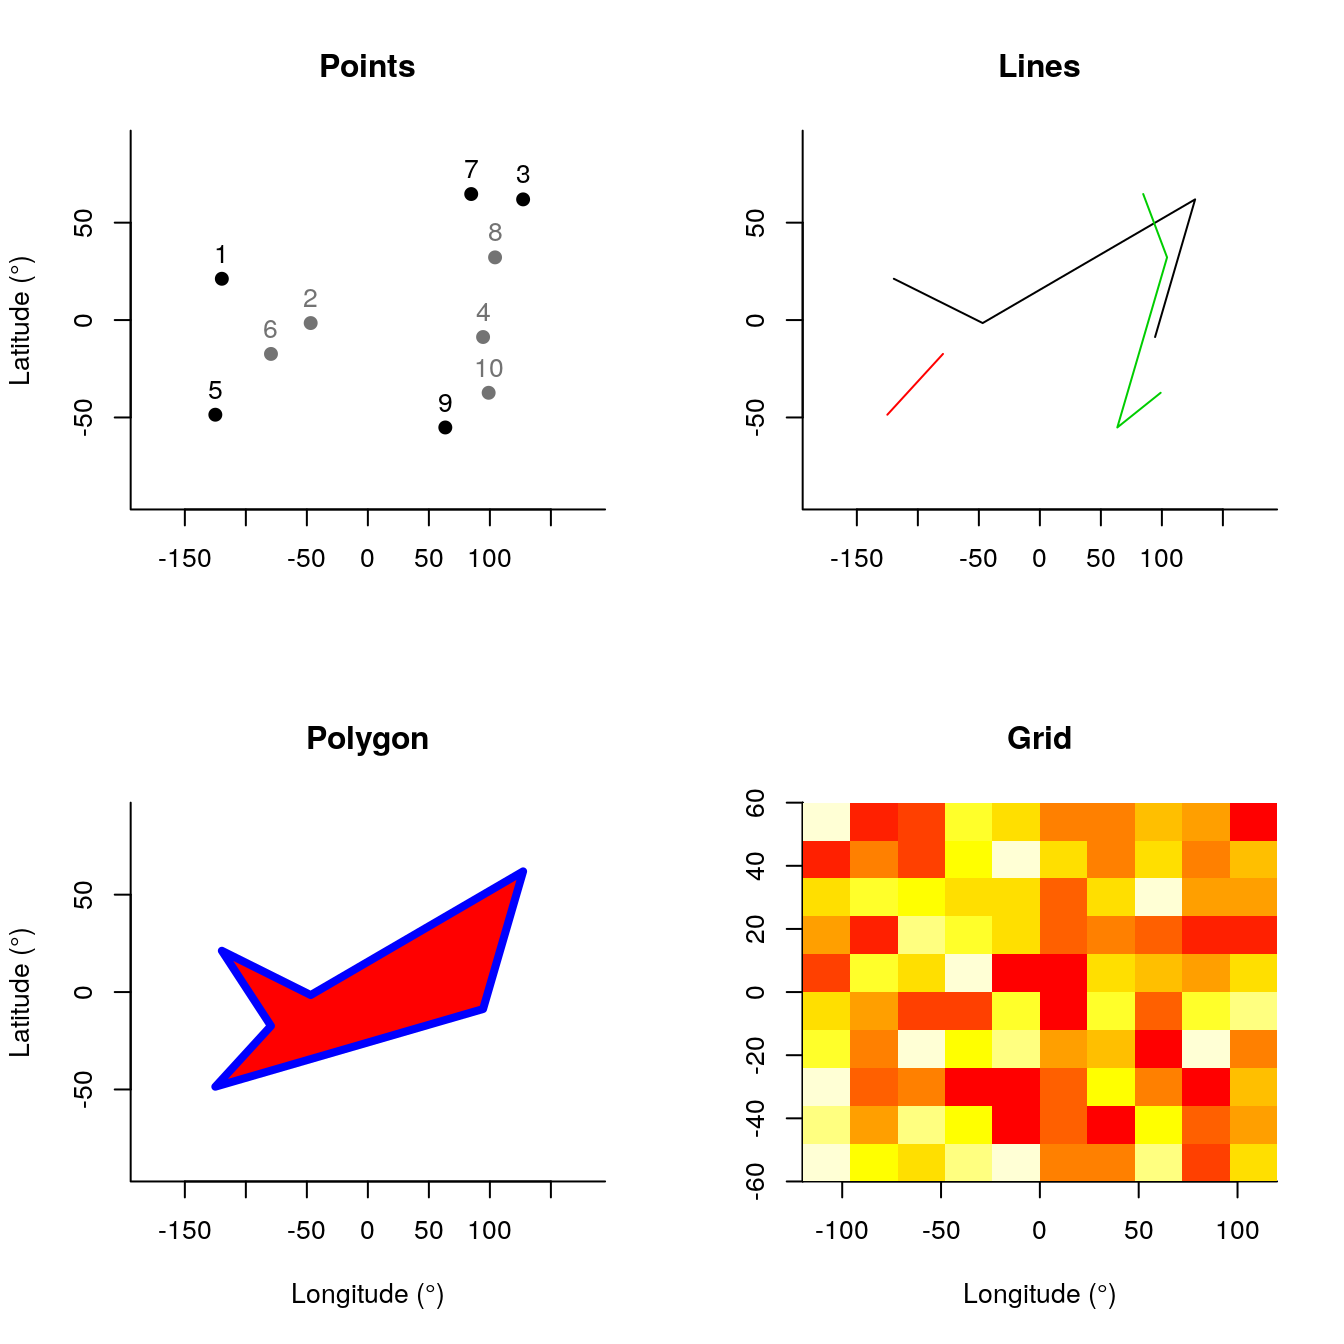
\includegraphics{mapsR_files/figure-latex/unnamed-chunk-6-1.pdf}
\caption{\label{fig1}Points, lines, polygons and grids. These are the
basic object manipulated when drawing maps.}
\end{figure}

\chapter{Classes for spatial objects in
R}\label{classes-for-spatial-objects-in-r}

\section{\texorpdfstring{The ``sp''
package}{The sp package}}\label{the-sp-package}

Manipulating efficiently spatial data requires more than graphical
skills. Indeed, spatial operations often involve to associate spatial
objects with datasets or with a Coordinate Reference System (CRS). To
provide a consistent framework to work with spatial objects in R, the
``sp'' package defines adequate classes and methods. These classes of
spatial objects are used by other packages (such as ``rgdal'', ``rgeos''
and ``raster'' that are used below) which makes R a powerful GIS:

\begin{Shaded}
\begin{Highlighting}[]
\KeywordTok{install.packages}\NormalTok{(}\StringTok{"sp"}\NormalTok{)}
\end{Highlighting}
\end{Shaded}

The documentation of this package and any package found on the
\href{http://cran.r-project.org/doc/manuals/r-release/R-intro.html}{CRAN
website} is available as a pdf file. For the ``sp'' package, you can
either look at the
\href{http://cran.r-project.org/web/packages/sp/index.html}{reference
manual} on line or you can enter the following command line in your R
console:

\begin{Shaded}
\begin{Highlighting}[]
\KeywordTok{library}\NormalTok{(}\DataTypeTok{help=}\StringTok{"sp"}\NormalTok{)}
\end{Highlighting}
\end{Shaded}

Then I load the package\footnote{Loading a package prevents you from
  using the name space of the package, ``sp::'' for ``sp'' package,
  before each function.}:

\begin{Shaded}
\begin{Highlighting}[]
\KeywordTok{library}\NormalTok{(}\StringTok{"sp"}\NormalTok{)}
\end{Highlighting}
\end{Shaded}

The ``sp'' package is the core package to turn R into a powerful
GIS\footnote{Contributed packages extent a lot R functionalities. The
  number of \href{https://cran.r-project.org/web/packages/}{contributed
  package} increases exponentially since its first release (June 2000);
  on the August 12, 2015, 7002 contributed packages were available.} and
the other packages that will be used depend on it. The table below
present the spatial classes that are used in this document. To create an
object of any of those classes, the function to be called is named after
the class of object it returns.

\begin{longtable}[]{@{}ll@{}}
\caption{Summary of the spatial classes defined by the ``sp'' package
that will be detail in this document.}\tabularnewline
\toprule
Classes / Functions & Contents\tabularnewline
\midrule
\endfirsthead
\toprule
Classes / Functions & Contents\tabularnewline
\midrule
\endhead
Points & list of points (set of coordinates)\tabularnewline
SpatialPoints & list of points + CRS\tabularnewline
SpatialPointsDataPoints & list of points + CRS + attribute
table\tabularnewline
Line & a line (set of coordinates)\tabularnewline
Lines & list of lines\tabularnewline
SpatialLines & list of lines + CRS\tabularnewline
SpatialLinesDataFrame & list of lines + CRS + attribute
table\tabularnewline
Polygon & a polygon (set of coordinates)\tabularnewline
Polygons & list of polygons\tabularnewline
SpatialPolygons & list of polygons + CRS\tabularnewline
SpatialPolygonsDataFrame & list of polygons + CRS + attribute
table\tabularnewline
GridTopology & Grid (smallest coordinates + cell size and
number)\tabularnewline
SpatialGrids & Grid + CRS\tabularnewline
SpatialGridsDataFrame & Grid + CRS + attribute table\tabularnewline
\bottomrule
\end{longtable}

\section{Spatial points}\label{spatial-points}

\subsection{\texorpdfstring{Class
\emph{SpatialPoints}}{Class SpatialPoints}}\label{class-spatialpoints}

Now, I re-use the coordinates that \textbf{vec} countains and I call the
\textbf{SpatialPoints()} function to get an object of class
\emph{SpatialPoints}.

\begin{Shaded}
\begin{Highlighting}[]
\NormalTok{ptsp <-}\StringTok{ }\KeywordTok{SpatialPoints}\NormalTok{(vec)}
\KeywordTok{print}\NormalTok{(ptsp)}
\end{Highlighting}
\end{Shaded}

\begin{verbatim}
## class       : SpatialPoints 
## features    : 10 
## extent      : -125.4915, 153.1097, -47.04658, 79.84521  (xmin, xmax, ymin, ymax)
## coord. ref. : NA
\end{verbatim}

Hence, an object of class \emph{SpatialPoints} is created. You may have
noticed that no CRS is defined. At this stage, it is optional. It can be
defined with the \emph{proj4string} that is encountered each time a CRS
can be associate a CRS to your object. Note that the way it actually
works is detailed in section {[}The ``rgdal'' package{]}{[}{]}. Below, I
specify that longitude and latitude will be used together with the
\href{http://en.wikipedia.org/wiki/Geodetic_datum}{geodetic datum} WGS84
(the most common).

\begin{Shaded}
\begin{Highlighting}[]
\NormalTok{ptsp <-}\StringTok{ }\KeywordTok{SpatialPoints}\NormalTok{(vec, }\DataTypeTok{proj4string=}\KeywordTok{CRS}\NormalTok{(}\StringTok{"+proj=longlat +datum=WGS84 +ellps=WGS84"}\NormalTok{))}
\KeywordTok{print}\NormalTok{(ptsp)}
\end{Highlighting}
\end{Shaded}

\begin{verbatim}
## class       : SpatialPoints 
## features    : 10 
## extent      : -125.4915, 153.1097, -47.04658, 79.84521  (xmin, xmax, ymin, ymax)
## coord. ref. : +proj=longlat +datum=WGS84 +ellps=WGS84 +towgs84=0,0,0
\end{verbatim}

\begin{Shaded}
\begin{Highlighting}[]
\KeywordTok{plot}\NormalTok{(ptsp)}
\end{Highlighting}
\end{Shaded}

\begin{figure}[htbp]
\centering
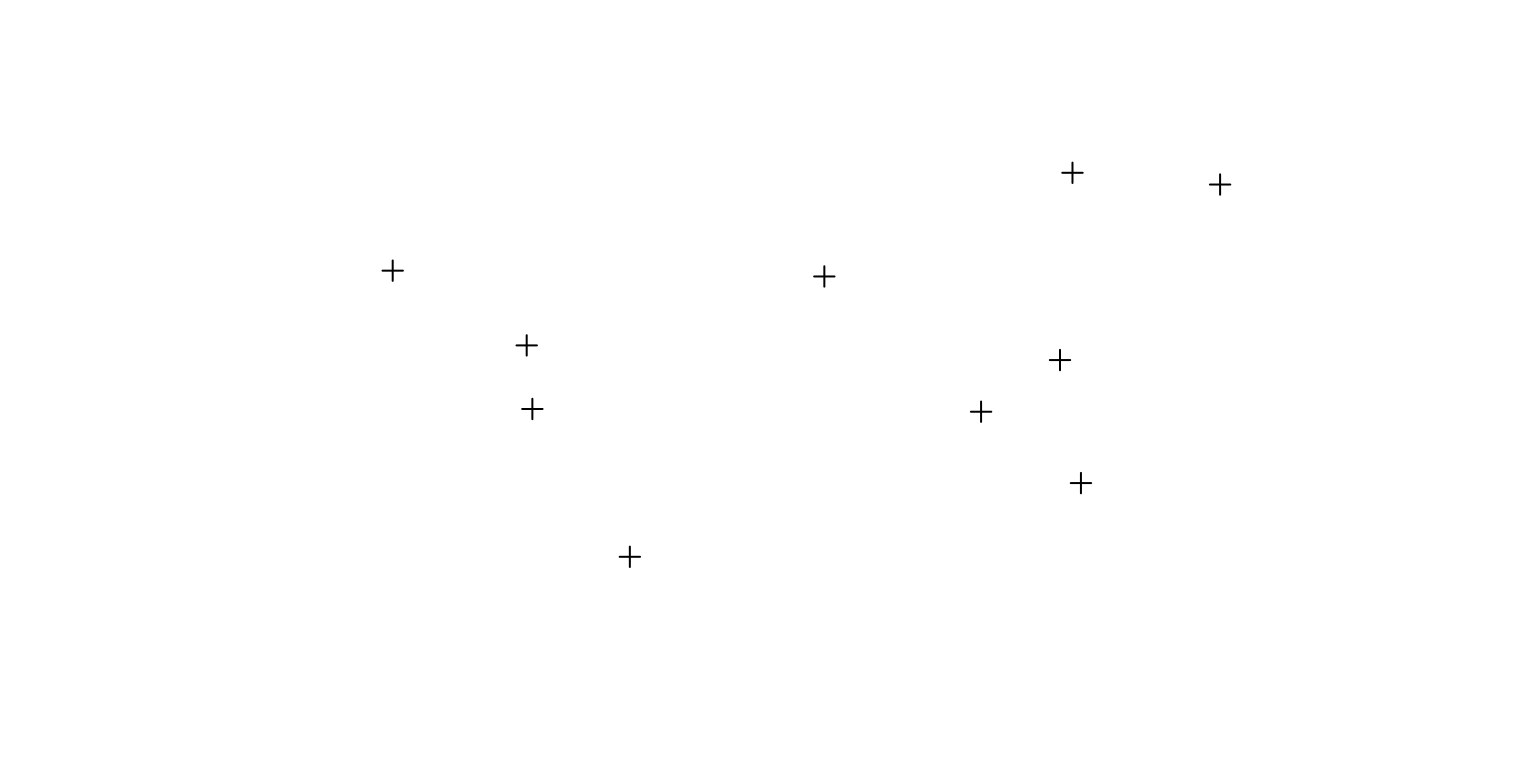
\includegraphics{mapsR_files/figure-latex/unnamed-chunk-11-1.pdf}
\caption{Spatial points and the default plot associated.}
\end{figure}

This plot differs from the one drawn in the previous section! This is
because there is a specific \textbf{plot()} method for spatial
object\footnote{To list all the different \textbf{plot()} methods, you
  can enter ``methods(plot)'' in the R console.}. This method is very
helpful, especially the \emph{add} argument that allows us to add
spatial objects on a base map. Now, I get a closer look at the
newly-defined spatial object.

\begin{Shaded}
\begin{Highlighting}[]
\KeywordTok{isS4}\NormalTok{(ptsp)}
\end{Highlighting}
\end{Shaded}

\begin{verbatim}
## [1] TRUE
\end{verbatim}

\begin{Shaded}
\begin{Highlighting}[]
\KeywordTok{structure}\NormalTok{(ptsp)}
\end{Highlighting}
\end{Shaded}

\begin{verbatim}
## class       : SpatialPoints 
## features    : 10 
## extent      : -125.4915, 153.1097, -47.04658, 79.84521  (xmin, xmax, ymin, ymax)
## coord. ref. : +proj=longlat +datum=WGS84 +ellps=WGS84 +towgs84=0,0,0
\end{verbatim}

It is a S4 object\footnote{Roughly speaking, objects in R are of two
  different kinds: S3 and S4. The first one is somehow more flexible
  while the latter is more formal. For more details, I recommend you to
  read \href{http://adv-r.had.co.nz/OO-essentials.html}{what Hadley
  Wickham wrote about it}.}, let's look at its attributes:

\begin{Shaded}
\begin{Highlighting}[]
\KeywordTok{attributes}\NormalTok{(ptsp)}
\end{Highlighting}
\end{Shaded}

\begin{verbatim}
## $bbox
##          min       max
## x -125.49155 153.10968
## y  -47.04658  79.84521
## 
## $proj4string
## CRS arguments:
##  +proj=longlat +datum=WGS84 +ellps=WGS84 +towgs84=0,0,0 
## 
## $coords
##                x         y
##  [1,]   80.83201  55.22742
##  [2,]  -99.65846  79.84521
##  [3,]  153.10968  55.90835
##  [4,] -125.49155 -47.04658
##  [5,]  -31.07683 -40.93509
##  [6,]   67.76399  31.96511
##  [7,] -112.30356  57.67134
##  [8,]   84.88552  24.45616
##  [9,]  116.61688 -41.56387
## [10,]   68.40036 -16.61647
## 
## $class
## [1] "SpatialPoints"
## attr(,"package")
## [1] "sp"
\end{verbatim}

One way to access to these attributes is given below:

\begin{Shaded}
\begin{Highlighting}[]
\CommentTok{# Let's call ptsp's extent}
\KeywordTok{attributes}\NormalTok{(ptsp)$bbox}
\end{Highlighting}
\end{Shaded}

\begin{verbatim}
##          min       max
## x -125.49155 153.10968
## y  -47.04658  79.84521
\end{verbatim}

Some attributes are slots that can be called using ``@'':

\begin{Shaded}
\begin{Highlighting}[]
\KeywordTok{slotNames}\NormalTok{(ptsp)}
\end{Highlighting}
\end{Shaded}

\begin{verbatim}
## [1] "coords"      "bbox"        "proj4string"
\end{verbatim}

\begin{Shaded}
\begin{Highlighting}[]
\CommentTok{# Let's call ptsp's proj4string}
\NormalTok{ptsp@proj4string}
\end{Highlighting}
\end{Shaded}

\begin{verbatim}
## CRS arguments:
##  +proj=longlat +datum=WGS84 +ellps=WGS84 +towgs84=0,0,0
\end{verbatim}

This is a powerful way to access any piece of information that spatial
objects contain.

\subsection{\texorpdfstring{Class
\emph{SpatialPointsDataFrame}}{Class SpatialPointsDataFrame}}\label{class-spatialpointsdataframe}

In spatial analysis, data may be associated with coordinates. For
vectors, data are stored in an attribute table. For instance, consider
you have geographic coordinates for different points corresponding to
different soil sample. To store the soil organic matter and/or the
percentage of clay associated to each sample, an attribute table must be
created. In R, creating a data is very straightforward thanks to the
\textbf{data.frame()} that creates \emph{data.frame} object:

\begin{Shaded}
\begin{Highlighting}[]
\CommentTok{# Brackets are used to print the table.}
\NormalTok{(datapt <-}\StringTok{ }\KeywordTok{data.frame}\NormalTok{(}\KeywordTok{cbind}\NormalTok{(}\DataTypeTok{Var1=}\KeywordTok{rnorm}\NormalTok{(nbp), }\DataTypeTok{Var2=}\DecValTok{1}\NormalTok{+}\KeywordTok{runif}\NormalTok{(nbp,}\DecValTok{0}\NormalTok{,}\DecValTok{10}\NormalTok{))))}
\end{Highlighting}
\end{Shaded}

\begin{verbatim}
##          Var1     Var2
## 1  -0.4945047 6.584873
## 2   0.2983024 5.381871
## 3  -0.0177299 9.938525
## 4   1.4862543 7.142660
## 5   0.6769118 5.705279
## 6  -1.7421249 2.695963
## 7  -2.7290769 2.186586
## 8  -0.3830236 4.976387
## 9   0.3721812 1.710268
## 10 -0.3167984 6.738220
\end{verbatim}

Given one \emph{SpatialPoints} object together with one
\emph{data.frame}, I create a \emph{SpatialPointsDataframe} object. It
contains all attributes you can find in a
\href{https://en.wikipedia.org/wiki/Shapefile}{Shapefile} of points.

\begin{Shaded}
\begin{Highlighting}[]
\NormalTok{ptspd <-}\StringTok{ }\KeywordTok{SpatialPointsDataFrame}\NormalTok{(ptsp, }\DataTypeTok{data=}\NormalTok{datapt)}
\KeywordTok{structure}\NormalTok{(ptspd)}
\end{Highlighting}
\end{Shaded}

\begin{verbatim}
## class       : SpatialPointsDataFrame 
## features    : 10 
## extent      : -125.4915, 153.1097, -47.04658, 79.84521  (xmin, xmax, ymin, ymax)
## coord. ref. : +proj=longlat +datum=WGS84 +ellps=WGS84 +towgs84=0,0,0 
## variables   : 2
## names       :              Var1,             Var2 
## min values  : -2.72907689693796, 1.71026777615771 
## max values  :  1.48625432667749, 9.93852484878153
\end{verbatim}

Our \textbf{datapt} is now the attribute table of \textbf{ptspd}. I can
efficiently access to the coordinates and the attributes tables using
\href{mailto:\%22@\%22}{\nolinkurl{"@"}}:

\begin{Shaded}
\begin{Highlighting}[]
\NormalTok{ptspd@data}
\end{Highlighting}
\end{Shaded}

\begin{verbatim}
##          Var1     Var2
## 1  -0.4945047 6.584873
## 2   0.2983024 5.381871
## 3  -0.0177299 9.938525
## 4   1.4862543 7.142660
## 5   0.6769118 5.705279
## 6  -1.7421249 2.695963
## 7  -2.7290769 2.186586
## 8  -0.3830236 4.976387
## 9   0.3721812 1.710268
## 10 -0.3167984 6.738220
\end{verbatim}

\begin{Shaded}
\begin{Highlighting}[]
\NormalTok{ptspd@coords}
\end{Highlighting}
\end{Shaded}

\begin{verbatim}
##                x         y
##  [1,]   80.83201  55.22742
##  [2,]  -99.65846  79.84521
##  [3,]  153.10968  55.90835
##  [4,] -125.49155 -47.04658
##  [5,]  -31.07683 -40.93509
##  [6,]   67.76399  31.96511
##  [7,] -112.30356  57.67134
##  [8,]   84.88552  24.45616
##  [9,]  116.61688 -41.56387
## [10,]   68.40036 -16.61647
\end{verbatim}

I plot \textbf{ptspd} and I specify that the size of points depends on
the second variable of the attribute table:

\begin{Shaded}
\begin{Highlighting}[]
\KeywordTok{plot}\NormalTok{(ptspd, }\DataTypeTok{pch=}\DecValTok{1}\NormalTok{, }\DataTypeTok{cex=}\NormalTok{ptspd@data$Var2)}
\end{Highlighting}
\end{Shaded}

\begin{figure}[htbp]
\centering
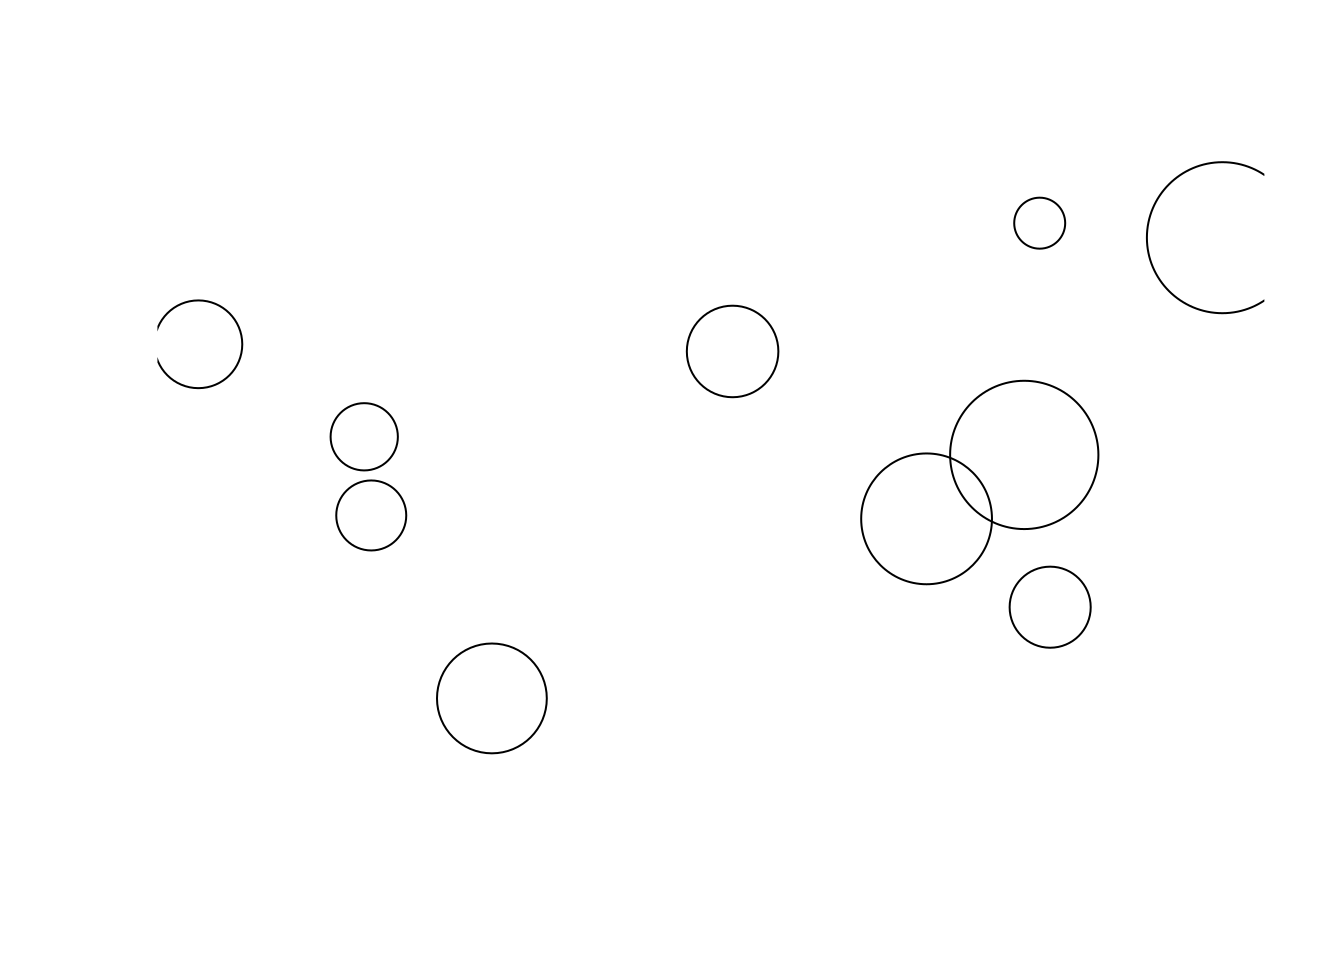
\includegraphics{mapsR_files/figure-latex/unnamed-chunk-19-1.pdf}
\caption{A simple but customized plot of the
\emph{SpatialPointsDataframe} object \textbf{ptspd}.}
\end{figure}

Among the advantage of these spatial classes, there is the easiness of
the definition of proper subsets. For instance, you can create a new
\emph{SpatialPointsDataFrame} with points 1,2,4,5,7,8 of the previous as
follows:

\begin{Shaded}
\begin{Highlighting}[]
\NormalTok{ptspd2 <-ptspd[}\KeywordTok{c}\NormalTok{(}\DecValTok{1}\NormalTok{,}\DecValTok{2}\NormalTok{,}\DecValTok{4}\NormalTok{,}\DecValTok{5}\NormalTok{,}\DecValTok{7}\NormalTok{,}\DecValTok{8}\NormalTok{),]}
\CommentTok{# or ptspd2 <-ptspd[-c(3,6,9,10),]}
\end{Highlighting}
\end{Shaded}

Consistently, I get:

\begin{Shaded}
\begin{Highlighting}[]
\KeywordTok{summary}\NormalTok{(ptspd2)}
\end{Highlighting}
\end{Shaded}

\begin{verbatim}
## Object of class SpatialPointsDataFrame
## Coordinates:
##          min      max
## x -125.49155 84.88552
## y  -47.04658 79.84521
## Is projected: FALSE 
## proj4string :
## [+proj=longlat +datum=WGS84 +ellps=WGS84 +towgs84=0,0,0]
## Number of points: 6
## Data attributes:
##       Var1               Var2      
##  Min.   :-2.72908   Min.   :2.187  
##  1st Qu.:-0.46663   1st Qu.:5.078  
##  Median :-0.04236   Median :5.544  
##  Mean   :-0.19086   Mean   :5.330  
##  3rd Qu.: 0.58226   3rd Qu.:6.365  
##  Max.   : 1.48625   Max.   :7.143
\end{verbatim}

\begin{Shaded}
\begin{Highlighting}[]
\NormalTok{ptspd2@data}
\end{Highlighting}
\end{Shaded}

\begin{verbatim}
##         Var1     Var2
## 1 -0.4945047 6.584873
## 2  0.2983024 5.381871
## 4  1.4862543 7.142660
## 5  0.6769118 5.705279
## 7 -2.7290769 2.186586
## 8 -0.3830236 4.976387
\end{verbatim}

The main benefit of using such classes is to manipulate efficiently
spatial objects. There are a lot of functions already implemented and it
is straightforward to automate basic operations. For instance, you can
get all the distance between your points as follows:

\begin{Shaded}
\begin{Highlighting}[]
\CommentTok{# spDists(ptspd2)}
\end{Highlighting}
\end{Shaded}

\section{Spatial Lines and Polygons}\label{spatial-lines-and-polygons}

Creating either spatial points, either spatial lines or spatial polygons
are essentially the same approach. In the last section, I show how to
create spatial points, so, for lines and polygon, instead of points,
fundamental units are lists of lines or polygons. Therefore, the first
step is to define these new units thanks to two functions:
\textbf{Line()} and \textbf{Polygon()}. As for points, I re-use objects
defined in the first section. Our lines are split into two groups of
lines. First, I create empty lists:

\begin{Shaded}
\begin{Highlighting}[]
\CommentTok{# Two lists for the lines.}
\NormalTok{li1 <-}\StringTok{ }\KeywordTok{list}\NormalTok{()}
\NormalTok{li2 <-}\StringTok{ }\KeywordTok{list}\NormalTok{()}
\CommentTok{# One for the polygons (it could have been more!).}
\NormalTok{pol1 <-}\StringTok{ }\KeywordTok{list}\NormalTok{()}
\end{Highlighting}
\end{Shaded}

Second, I fill the empty list using \textbf{Line()} and
\textbf{Polygon()} to create the fundamental units.

\begin{Shaded}
\begin{Highlighting}[]
\NormalTok{li1[[}\DecValTok{1}\NormalTok{]]<-}\StringTok{ }\KeywordTok{Line}\NormalTok{(}\KeywordTok{cbind}\NormalTok{(vec$x[}\DecValTok{1}\NormalTok{:}\DecValTok{4}\NormalTok{], vec$y[}\DecValTok{1}\NormalTok{:}\DecValTok{4}\NormalTok{]))}
\NormalTok{li1[[}\DecValTok{2}\NormalTok{]]<-}\StringTok{ }\KeywordTok{Line}\NormalTok{(}\KeywordTok{cbind}\NormalTok{(vec$x[}\DecValTok{5}\NormalTok{:}\DecValTok{6}\NormalTok{], vec$y[}\DecValTok{5}\NormalTok{:}\DecValTok{6}\NormalTok{]))}
\NormalTok{##}
\NormalTok{li2[[}\DecValTok{1}\NormalTok{]]<-}\StringTok{ }\KeywordTok{Line}\NormalTok{(}\KeywordTok{cbind}\NormalTok{(vec$x[}\DecValTok{7}\NormalTok{:}\DecValTok{10}\NormalTok{], vec$y[}\DecValTok{7}\NormalTok{:}\DecValTok{10}\NormalTok{]))}
\NormalTok{####}
\NormalTok{pol1[[}\DecValTok{1}\NormalTok{]] <-}\StringTok{ }\KeywordTok{Polygon}\NormalTok{(}\KeywordTok{cbind}\NormalTok{(}\KeywordTok{c}\NormalTok{(vec$x[}\DecValTok{1}\NormalTok{:}\DecValTok{6}\NormalTok{],vec$x[}\DecValTok{1}\NormalTok{]), }\KeywordTok{c}\NormalTok{(vec$y[}\DecValTok{1}\NormalTok{:}\DecValTok{6}\NormalTok{],vec$y[}\DecValTok{1}\NormalTok{])))}
\end{Highlighting}
\end{Shaded}

The next step transforms the previous lists into \emph{Lines} and
\emph{Polygons} object that must be identifies with an unique ID for the
next building steps.

\begin{Shaded}
\begin{Highlighting}[]
\NormalTok{lin1 <-}\StringTok{ }\KeywordTok{Lines}\NormalTok{(li1,}\DataTypeTok{ID=}\DecValTok{1}\NormalTok{)}
\NormalTok{lin2 <-}\StringTok{ }\KeywordTok{Lines}\NormalTok{(li2,}\DataTypeTok{ID=}\DecValTok{2}\NormalTok{)}
\NormalTok{##}
\NormalTok{poly1 <-}\StringTok{  }\KeywordTok{Polygons}\NormalTok{(pol1, }\DataTypeTok{ID=}\DecValTok{1}\NormalTok{)}
\end{Highlighting}
\end{Shaded}

Then, I define object of class \emph{SpatialLines} and
\emph{SpatialPolygons}. They are respectively made of lists of lists of
lines and polygons together with a CRS.

\begin{Shaded}
\begin{Highlighting}[]
\NormalTok{linsp <-}\StringTok{ }\KeywordTok{SpatialLines}\NormalTok{(}\KeywordTok{list}\NormalTok{(lin1,lin2),}
    \DataTypeTok{proj4string=}\KeywordTok{CRS}\NormalTok{(}\StringTok{"+proj=longlat +datum=WGS84 +ellps=WGS84"}\NormalTok{))}
\CommentTok{#}
\NormalTok{polsp <-}\StringTok{ }\KeywordTok{SpatialPolygons}\NormalTok{(}\KeywordTok{list}\NormalTok{(poly1),}
    \DataTypeTok{proj4string=}\KeywordTok{CRS}\NormalTok{(}\StringTok{"+proj=longlat +datum=WGS84 +ellps=WGS84"}\NormalTok{))}
\end{Highlighting}
\end{Shaded}

Finally, I add an attribute table to obtain objects of class
\emph{SpatialLinesDataFrame} and \emph{SpatialPolygonsDataFrame}.

\begin{Shaded}
\begin{Highlighting}[]
\NormalTok{datalin<-}\KeywordTok{data.frame}\NormalTok{(}\DataTypeTok{var1=}\KeywordTok{runif}\NormalTok{(}\DecValTok{2}\NormalTok{), }\DataTypeTok{var2=}\KeywordTok{rnorm}\NormalTok{(}\DecValTok{2}\NormalTok{), }\DataTypeTok{var3=}\KeywordTok{rpois}\NormalTok{(}\DecValTok{2}\NormalTok{,}\DecValTok{10}\NormalTok{))}
\NormalTok{linspd <-}\StringTok{ }\KeywordTok{SpatialLinesDataFrame}\NormalTok{(linsp, }\DataTypeTok{data=}\KeywordTok{as.data.frame}\NormalTok{(datalin))}
\CommentTok{#}
\NormalTok{datapol<-}\KeywordTok{data.frame}\NormalTok{(}\DataTypeTok{var1=}\KeywordTok{runif}\NormalTok{(}\DecValTok{1}\NormalTok{), }\DataTypeTok{var2=}\KeywordTok{rnorm}\NormalTok{(}\DecValTok{1}\NormalTok{), }\DataTypeTok{var3=}\KeywordTok{rpois}\NormalTok{(}\DecValTok{1}\NormalTok{,}\DecValTok{10}\NormalTok{))}
\NormalTok{polspd <-}\StringTok{ }\KeywordTok{SpatialPolygonsDataFrame}\NormalTok{(polsp, }\DataTypeTok{data=}\NormalTok{datapol)}
\end{Highlighting}
\end{Shaded}

I suggest you look at these objects using \textbf{attributes()} or
\textbf{structures()} functions. To conclude the section, let's make a
quick plot:

\begin{Shaded}
\begin{Highlighting}[]
\KeywordTok{par}\NormalTok{(}\DataTypeTok{mfrow=}\KeywordTok{c}\NormalTok{(}\DecValTok{1}\NormalTok{,}\DecValTok{2}\NormalTok{), }\DataTypeTok{ann=}\OtherTok{FALSE}\NormalTok{, }\DataTypeTok{bty=}\StringTok{"l"}\NormalTok{)}
\KeywordTok{plot}\NormalTok{(linspd, }\DataTypeTok{col=}\KeywordTok{c}\NormalTok{(}\DecValTok{2}\NormalTok{,}\DecValTok{4}\NormalTok{))}
\KeywordTok{plot}\NormalTok{(polspd, }\DataTypeTok{col=}\DecValTok{4}\NormalTok{)}
\end{Highlighting}
\end{Shaded}

\begin{figure}[htbp]
\centering
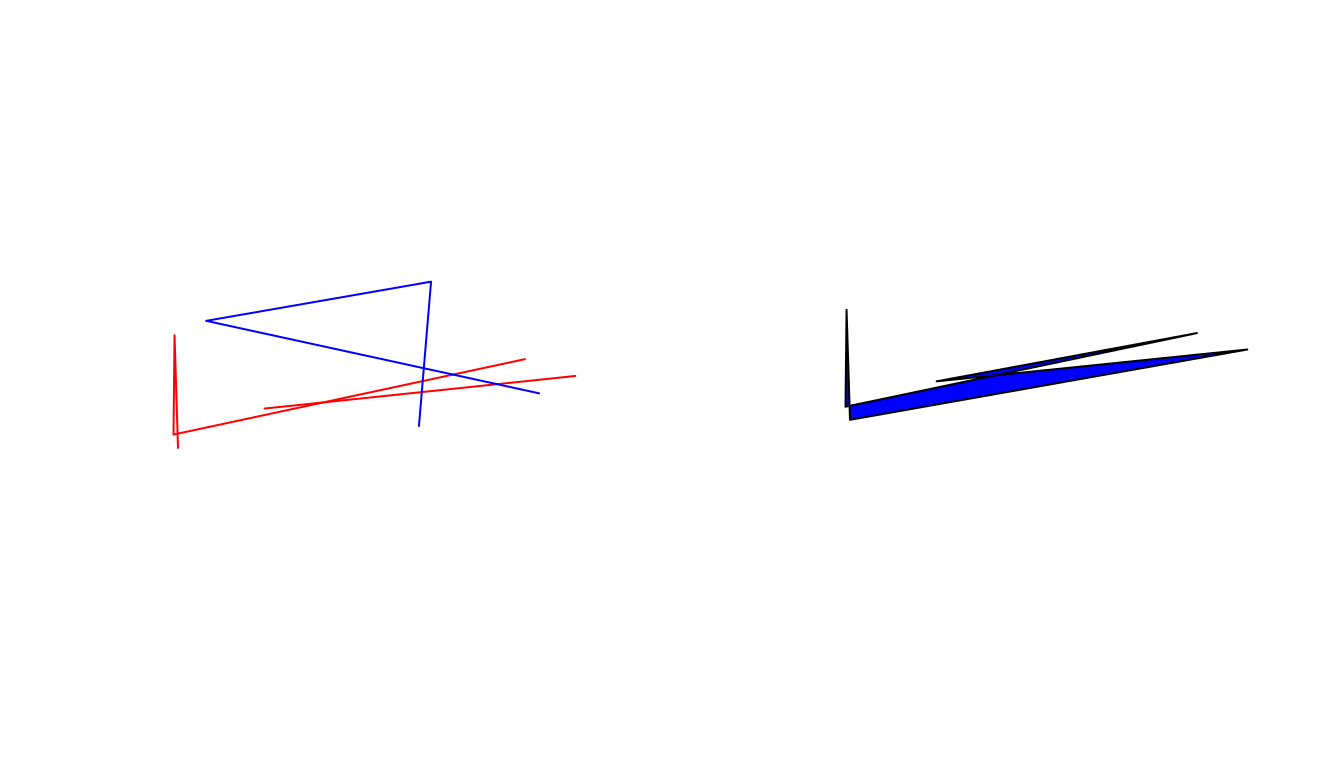
\includegraphics{mapsR_files/figure-latex/unnamed-chunk-28-1.pdf}
\caption{\emph{SpatialLines} (on the left) and \emph{SpatialPolygons}
(on the right).}
\end{figure}

\chapter{Spatial grids}\label{spatial-grids}

The last classes of spatial defined in the ``sp'' package to be
presented are grids. Here, I do not present how to use a
\emph{SpatialPixel}. Rather, I shortly focus on \emph{SpatialGrid}
objects. Note that the next chapter is dedicated to raster objects which
are more used (as far as I know). First, you need to define a grid
topology using the \textbf{GridTopology()} function. You must specify
the following arguments:

\begin{enumerate}
\def\labelenumi{\arabic{enumi}.}
\tightlist
\item
  \emph{cellcentre.offset}: coordinates of the centre of the bottom-left
\item
  \emph{cellsize}: a vector with the cell size in each dimension.
\item
  \emph{cells.dim}: a vector with the number of cells in each dimension.
\end{enumerate}

\begin{Shaded}
\begin{Highlighting}[]
\NormalTok{grd <-}\StringTok{ }\KeywordTok{GridTopology}\NormalTok{(}\DataTypeTok{cellcentre.offset=}\KeywordTok{c}\NormalTok{(-}\FloatTok{179.5}\NormalTok{,-}\FloatTok{89.5}\NormalTok{), }\DataTypeTok{cellsize=}\KeywordTok{c}\NormalTok{(}\DecValTok{1}\NormalTok{,}\DecValTok{1}\NormalTok{), }\DataTypeTok{cells.dim=}\KeywordTok{c}\NormalTok{(}\DecValTok{360}\NormalTok{,}\DecValTok{180}\NormalTok{))}
\end{Highlighting}
\end{Shaded}

Then, I create a \emph{SpatialGrid} by adding a CRS:

\begin{Shaded}
\begin{Highlighting}[]
\NormalTok{grdsp <-}\StringTok{ }\KeywordTok{SpatialGrid}\NormalTok{(grd, }\DataTypeTok{proj4string=}\KeywordTok{CRS}\NormalTok{(}\StringTok{"+proj=longlat +datum=WGS84 +ellps=WGS84"}\NormalTok{))}
\end{Highlighting}
\end{Shaded}

Finally, an attribute table is added to \textbf{grdsp} to obtain a
\emph{SpatialGridDataFrame} object called \textbf{grdspd}.

\begin{Shaded}
\begin{Highlighting}[]
\NormalTok{var1 <-}\StringTok{ }\KeywordTok{runif}\NormalTok{(}\DecValTok{360}\NormalTok{*}\DecValTok{180}\NormalTok{, }\DecValTok{0}\NormalTok{, }\DecValTok{10}\NormalTok{)}
\NormalTok{var2 <-}\StringTok{ }\KeywordTok{rnorm}\NormalTok{(}\DecValTok{360}\NormalTok{*}\DecValTok{180}\NormalTok{, }\DecValTok{0}\NormalTok{, }\DecValTok{10}\NormalTok{)}
\NormalTok{datagd <-}\StringTok{ }\KeywordTok{data.frame}\NormalTok{(var1, var2)}
\CommentTok{#}
\NormalTok{grdspd <-}\StringTok{ }\KeywordTok{SpatialGridDataFrame}\NormalTok{(grdsp, }\DataTypeTok{data=}\NormalTok{datagd)}
\KeywordTok{par}\NormalTok{(}\DataTypeTok{mar=}\KeywordTok{c}\NormalTok{(}\DecValTok{4}\NormalTok{,}\DecValTok{4}\NormalTok{,}\DecValTok{1}\NormalTok{,}\DecValTok{1}\NormalTok{))}
\end{Highlighting}
\end{Shaded}

I plot the new object and I add \textbf{ptspd} on it.

\begin{Shaded}
\begin{Highlighting}[]
\KeywordTok{image}\NormalTok{(grdspd)}
\KeywordTok{axis}\NormalTok{(}\DecValTok{1}\NormalTok{, }\KeywordTok{seq}\NormalTok{(-}\DecValTok{180}\NormalTok{, }\DecValTok{180}\NormalTok{, }\DataTypeTok{by=}\DecValTok{20}\NormalTok{))}
\KeywordTok{axis}\NormalTok{(}\DecValTok{2}\NormalTok{, }\KeywordTok{seq}\NormalTok{(-}\DecValTok{90}\NormalTok{, }\DecValTok{90}\NormalTok{, }\DataTypeTok{by=}\DecValTok{30}\NormalTok{))}
\KeywordTok{title}\NormalTok{(}\DataTypeTok{xlab=}\StringTok{"Longitude"}\NormalTok{, }\DataTypeTok{ylab=}\StringTok{"latitude"}\NormalTok{)}
\KeywordTok{plot}\NormalTok{(ptspd, }\DataTypeTok{add=}\OtherTok{TRUE}\NormalTok{)}
\end{Highlighting}
\end{Shaded}

\begin{figure}[htbp]
\centering
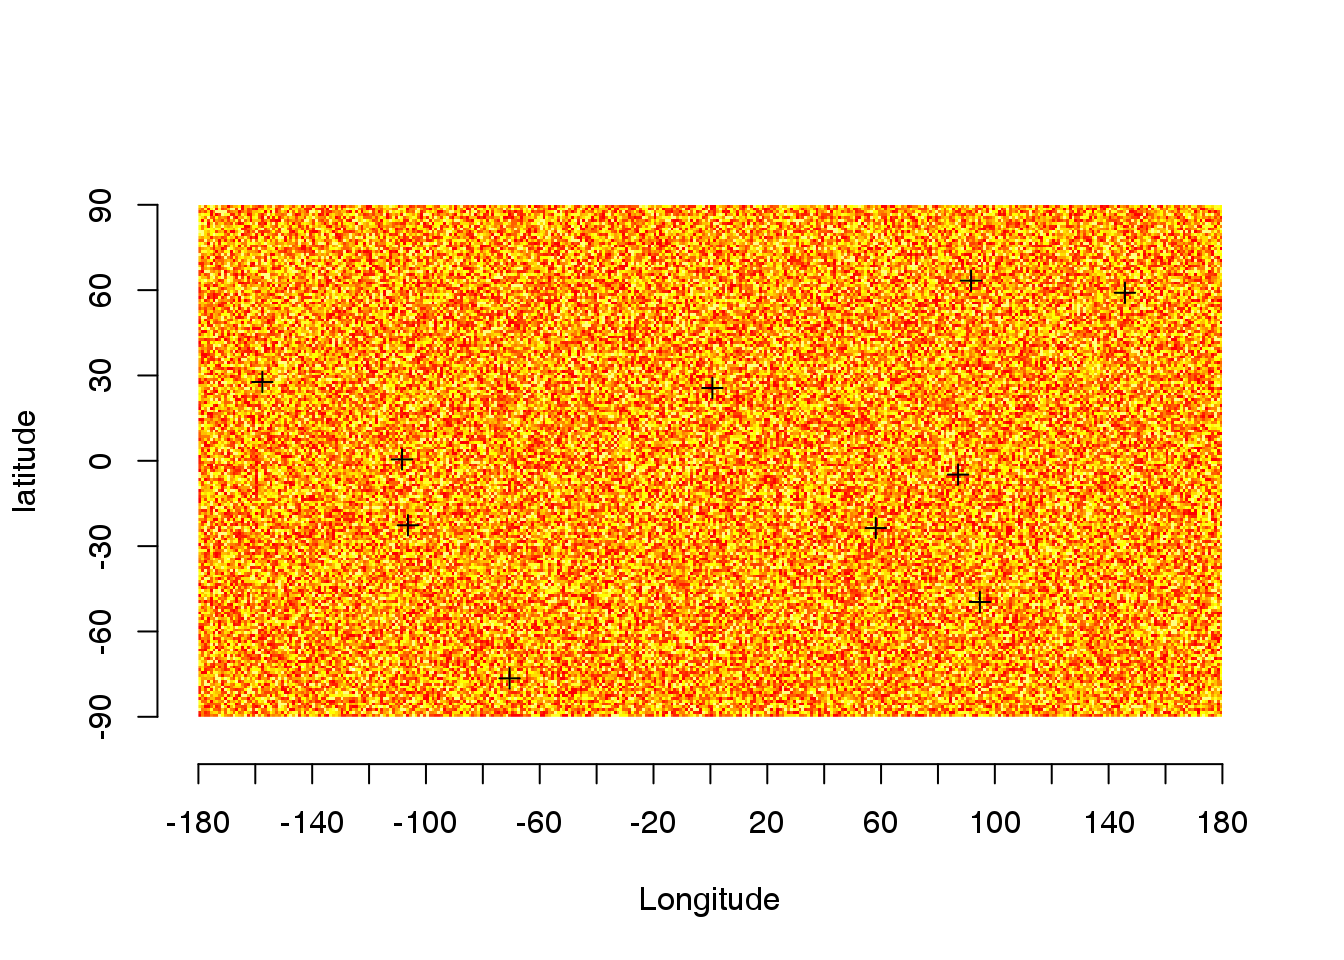
\includegraphics{mapsR_files/figure-latex/unnamed-chunk-32-1.pdf}
\caption{SpatialGrid plotted with the \emph{image} function together
with}
\end{figure}

\chapter{Rasters}\label{rasters}

\section{\texorpdfstring{Package
``raster''}{Package raster}}\label{package-raster}

The
\href{http://cran.r-project.org/web/packages/raster/raster.pdf}{``raster''
package} defines classes, methods and functions for raster files. To the
best of my knowledge, I feel that people more often work with this
package rather than with the classes for grids defined in the ``sp''
package (but ``raster'' still imports ``sp''). I personally use ``sp''
package to manipulate vector files and ``raster'' for raster formats.
First, let's install and the package.

\begin{Shaded}
\begin{Highlighting}[]
\KeywordTok{install.packages}\NormalTok{(}\StringTok{"raster"}\NormalTok{)}
\KeywordTok{library}\NormalTok{(raster)}
\end{Highlighting}
\end{Shaded}

In the following sections below, I introduce the different classes
defined in ``raster''; that is \emph{RasterLayer}, \emph{RasterStack}
and \emph{RasterBrick}.

\section{RasterLayer}\label{rasterlayer}

\subsection{\texorpdfstring{Function
\textbf{raster}}{Function raster}}\label{function-raster}

To create a first ``raster'' object, I call \textbf{raster} function. As
mentioned in the documentation of the function, they are many way to
build a \emph{RasterLayer}, notably:

1- a path to a raster file 2- a \emph{SpatialGrid}, defined as above 3-
a matrix 4- an object of class \emph{RasterLayer}, \emph{RasterStack} or
\emph{RasterBrick}

The first example I choose is creating a \emph{RasterLayer} from a
matrix (others are similar, see the documentation). To do so, I specify
the minimum and maximum centre coordinates in each dimension. The number
of cells in each dimension is provided by the number of rows and columns
of the matrix passed to the function.

\begin{Shaded}
\begin{Highlighting}[]
\NormalTok{Ra1 <-}\StringTok{ }\KeywordTok{raster}\NormalTok{(}\KeywordTok{matrix}\NormalTok{(}\KeywordTok{runif}\NormalTok{(}\DecValTok{360}\NormalTok{*}\DecValTok{180}\NormalTok{,}\DecValTok{0}\NormalTok{,}\DecValTok{10}\NormalTok{),}\DataTypeTok{ncol=}\DecValTok{360}\NormalTok{,}\DataTypeTok{nrow=}\DecValTok{180}\NormalTok{),}
    \DataTypeTok{crs=}\KeywordTok{CRS}\NormalTok{(}\StringTok{"+proj=longlat +datum=WGS84 +no_defs +ellps=WGS84 +towgs84=0,0,0"}\NormalTok{),}
    \DataTypeTok{xmn=}\NormalTok{-}\FloatTok{179.5}\NormalTok{, }\DataTypeTok{xmx=}\NormalTok{+}\FloatTok{179.5}\NormalTok{, }\DataTypeTok{ymn=}\NormalTok{-}\FloatTok{79.5}\NormalTok{, }\DataTypeTok{ymx=}\NormalTok{+}\FloatTok{79.5}\NormalTok{)}
\NormalTok{Ra1}
\end{Highlighting}
\end{Shaded}

\begin{verbatim}
## class       : RasterLayer 
## dimensions  : 180, 360, 64800  (nrow, ncol, ncell)
## resolution  : 0.9972222, 0.8833333  (x, y)
## extent      : -179.5, 179.5, -79.5, 79.5  (xmin, xmax, ymin, ymax)
## coord. ref. : +proj=longlat +datum=WGS84 +no_defs +ellps=WGS84 +towgs84=0,0,0 
## data source : in memory
## names       : layer 
## values      : 1.4666e-05, 9.999793  (min, max)
\end{verbatim}

I suggest you have a look on the attributes of the \emph{RasterLayer}
object defined using \textbf{structure} or \textbf{attributes} function.
Notably, you can visualize values using function \textbf{values}:

\begin{Shaded}
\begin{Highlighting}[]
\NormalTok{val1 <-}\StringTok{ }\KeywordTok{values}\NormalTok{(Ra1)}
\NormalTok{## I print the ten first values.}
\NormalTok{val1[}\DecValTok{1}\NormalTok{:}\DecValTok{10}\NormalTok{]}
\end{Highlighting}
\end{Shaded}

\begin{verbatim}
##  [1] 9.169142 8.757451 4.111959 3.681748 7.089988 4.058775 5.418238
##  [8] 7.988517 4.605570 4.048225
\end{verbatim}

You may have noticed that there is no ``proj4string'' argument but a CRS
argument. However it exists a common way to access the CRS for all the
spatial objects we are studying: function \textbf{projection}.

\begin{Shaded}
\begin{Highlighting}[]
\KeywordTok{projection}\NormalTok{(Ra1)}
\end{Highlighting}
\end{Shaded}

\begin{verbatim}
## [1] "+proj=longlat +datum=WGS84 +no_defs +ellps=WGS84 +towgs84=0,0,0"
\end{verbatim}

\begin{Shaded}
\begin{Highlighting}[]
\KeywordTok{projection}\NormalTok{(ptspd)}
\end{Highlighting}
\end{Shaded}

\begin{verbatim}
## [1] "+proj=longlat +datum=WGS84 +ellps=WGS84 +towgs84=0,0,0"
\end{verbatim}

Similarly, function \textbf{extent} provides a common way to get the
extent of spatial objects:

\begin{Shaded}
\begin{Highlighting}[]
\KeywordTok{extent}\NormalTok{(Ra1)}
\end{Highlighting}
\end{Shaded}

\begin{verbatim}
## class       : Extent 
## xmin        : -179.5 
## xmax        : 179.5 
## ymin        : -79.5 
## ymax        : 79.5
\end{verbatim}

\begin{Shaded}
\begin{Highlighting}[]
\KeywordTok{extent}\NormalTok{(ptspd)}
\end{Highlighting}
\end{Shaded}

\begin{verbatim}
## class       : Extent 
## xmin        : -125.4915 
## xmax        : 153.1097 
## ymin        : -47.04658 
## ymax        : 79.84521
\end{verbatim}

Note that using \emph{extent} object is also a convenient way to create
a \emph{RasterLayer}:

\begin{Shaded}
\begin{Highlighting}[]
\NormalTok{Ra2 <-}\StringTok{ }\KeywordTok{raster}\NormalTok{(}\KeywordTok{extent}\NormalTok{(Ra1), }\DataTypeTok{nrows=}\DecValTok{100}\NormalTok{, }\DataTypeTok{ncols=}\DecValTok{100}\NormalTok{, }\DataTypeTok{crs=}\KeywordTok{projection}\NormalTok{(Ra1))}
\NormalTok{Ra2}
\end{Highlighting}
\end{Shaded}

\begin{verbatim}
## class       : RasterLayer 
## dimensions  : 100, 100, 10000  (nrow, ncol, ncell)
## resolution  : 3.59, 1.59  (x, y)
## extent      : -179.5, 179.5, -79.5, 79.5  (xmin, xmax, ymin, ymax)
## coord. ref. : +proj=longlat +datum=WGS84 +no_defs +ellps=WGS84 +towgs84=0,0,0
\end{verbatim}

I now plot \emph{Ra1} using either \textbf{plot} or \textbf{image}. Note
that their default rendering differs.

\begin{Shaded}
\begin{Highlighting}[]
\KeywordTok{par}\NormalTok{(}\DataTypeTok{mfrow=}\KeywordTok{c}\NormalTok{(}\DecValTok{2}\NormalTok{,}\DecValTok{1}\NormalTok{))}
\KeywordTok{plot}\NormalTok{(Ra1)}
\KeywordTok{image}\NormalTok{(Ra1)}
\end{Highlighting}
\end{Shaded}

\begin{figure}[htbp]
\centering
\includegraphics{mapsR_files/figure-latex/unnamed-chunk-40-1.pdf}
\caption{Plot of a \emph{RasterLayer} object using \emph{plot} and
\emph{image} functions}
\end{figure}

The \textbf{raster} function is also a useful method to convert
\emph{SpatialGrid} to \emph{RasterLayer}.

\begin{Shaded}
\begin{Highlighting}[]
\NormalTok{Ra3 <-}\StringTok{ }\KeywordTok{raster}\NormalTok{(grdsp)}
\NormalTok{Ra3}
\end{Highlighting}
\end{Shaded}

\begin{verbatim}
## class       : RasterLayer 
## dimensions  : 180, 360, 64800  (nrow, ncol, ncell)
## resolution  : 1, 1  (x, y)
## extent      : -180, 180, -90, 90  (xmin, xmax, ymin, ymax)
## coord. ref. : +proj=longlat +datum=WGS84 +ellps=WGS84 +towgs84=0,0,0
\end{verbatim}

\subsection{\texorpdfstring{The \emph{rasterize}
function}{The rasterize function}}\label{the-rasterize-function}

Rasters can also be created based on vector object such as the one we
have previously scrutinized. To do so, you may use the
\textbf{rasterize} function and a ``RasterLayer''. The latter is used to
define the grid you want to use as a support.

\begin{Shaded}
\begin{Highlighting}[]
\CommentTok{# Points as raster.}
\NormalTok{Ra3 <-}\StringTok{ }\KeywordTok{rasterize}\NormalTok{(ptspd,Ra1)}
\CommentTok{# Lines as raster.}
\NormalTok{Ra4 <-}\StringTok{ }\KeywordTok{rasterize}\NormalTok{(linspd,Ra1)}
\NormalTok{val4 <-}\StringTok{ }\KeywordTok{values}\NormalTok{(Ra4)}
\CommentTok{# Polygons as raster.}
\NormalTok{Ra5 <-}\StringTok{ }\KeywordTok{rasterize}\NormalTok{(polsp,Ra1)}
\end{Highlighting}
\end{Shaded}

You can plot the raterized polygons as follows:

\begin{Shaded}
\begin{Highlighting}[]
\KeywordTok{image}\NormalTok{(Ra4)}
\end{Highlighting}
\end{Shaded}

\begin{figure}[htbp]
\centering
\includegraphics{mapsR_files/figure-latex/unnamed-chunk-43-1.pdf}
\caption{SpatialLinesDataFrame rasterized}
\end{figure}

Note that \textbf{rasterize} can also be used to create
\emph{rasterlayer} from matrix.

\section{RasterStacks and
RasterBricks}\label{rasterstacks-and-rasterbricks}

These classes deal with multi-layer raster objects. They are basically
similar but ``the processing time should be shorter when using a
RasterBrick''\footnote{Documentation of function ``brick''.}. Also,
RasterBricks ``are less flexible as they can only point to a single
file''\footnote{Documentation of function ``brick''.}. To create an
object of class \emph{RasterStacks}, one uses the function
\textbf{stack}. Similarly to create a \emph{RasterBricks} object, one
uses \textbf{brick}.

\begin{Shaded}
\begin{Highlighting}[]
\NormalTok{Ras1 <-}\StringTok{ }\KeywordTok{stack}\NormalTok{(Ra1, Ra3, Ra4)}
\NormalTok{Rab1 <-}\StringTok{ }\KeywordTok{brick}\NormalTok{(Ra1, Ra3, Ra4)}
\end{Highlighting}
\end{Shaded}

Let's have a look at the classes of the object:

\begin{Shaded}
\begin{Highlighting}[]
\KeywordTok{class}\NormalTok{(Ras1)}
\end{Highlighting}
\end{Shaded}

\begin{verbatim}
## [1] "RasterStack"
## attr(,"package")
## [1] "raster"
\end{verbatim}

\begin{Shaded}
\begin{Highlighting}[]
\KeywordTok{class}\NormalTok{(Rab1)}
\end{Highlighting}
\end{Shaded}

\begin{verbatim}
## [1] "RasterBrick"
## attr(,"package")
## [1] "raster"
\end{verbatim}

The numbers of layers is provided by function \textbf{nlayers}:

\begin{Shaded}
\begin{Highlighting}[]
\KeywordTok{nlayers}\NormalTok{(Ras1)}
\end{Highlighting}
\end{Shaded}

\begin{verbatim}
## [1] 5
\end{verbatim}

\begin{Shaded}
\begin{Highlighting}[]
\KeywordTok{nlayers}\NormalTok{(Rab1)}
\end{Highlighting}
\end{Shaded}

\begin{verbatim}
## [1] 5
\end{verbatim}

Note that you can also look at the class of the different layers:

\begin{Shaded}
\begin{Highlighting}[]
\KeywordTok{class}\NormalTok{(Ras1[[}\DecValTok{1}\NormalTok{]])}
\end{Highlighting}
\end{Shaded}

\begin{verbatim}
## [1] "RasterLayer"
## attr(,"package")
## [1] "raster"
\end{verbatim}

\begin{Shaded}
\begin{Highlighting}[]
\KeywordTok{class}\NormalTok{(Rab1[[}\DecValTok{1}\NormalTok{]])}
\end{Highlighting}
\end{Shaded}

\begin{verbatim}
## [1] "RasterLayer"
## attr(,"package")
## [1] "raster"
\end{verbatim}

Again, there is a plot method associated with these objects:

\begin{Shaded}
\begin{Highlighting}[]
\KeywordTok{plot}\NormalTok{(Ras1)}
\end{Highlighting}
\end{Shaded}

\begin{figure}[htbp]
\centering
\includegraphics{mapsR_files/figure-latex/unnamed-chunk-48-1.pdf}
\caption{Raster}
\end{figure}

\begin{Shaded}
\begin{Highlighting}[]
\KeywordTok{plot}\NormalTok{(Rab1)}
\end{Highlighting}
\end{Shaded}

\begin{figure}[htbp]
\centering
\includegraphics{mapsR_files/figure-latex/unnamed-chunk-49-1.pdf}
\caption{Raster}
\end{figure}

Function \textbf{unstack} permits the reverse operation, i.e.~getting a
list of \emph{RasterLayers} from \emph{RasterLayers} or
\emph{RasterBricks}:

\begin{Shaded}
\begin{Highlighting}[]
\NormalTok{liRa <-}\StringTok{ }\KeywordTok{unstack}\NormalTok{(Ras1)}
\end{Highlighting}
\end{Shaded}

\chapter{Import and export spatial
objects}\label{import-and-export-spatial-objects}

\section{\texorpdfstring{Package
``rgdal''}{Package rgdal}}\label{package-rgdal}

This package makes possible to handle many spatial formats. By doing so,
it turns R into a powerful spatial converter. Below, I focus on few
important functions of this package:

\begin{enumerate}
\def\labelenumi{\arabic{enumi}.}
\tightlist
\item
  \textbf{writeOGR} / \textbf{writeGDAL}: to write spatial objects.
\item
  \textbf{readOGR}/\textbf{readGDAL}: to read spatial files.
\item
  \textbf{spTransform}: to change geographical projection.
\end{enumerate}

This package takes advantage from the open-source
\href{http://www.gdal.org/index.html}{GDAL library} to read the
different formats and the cartographic projection library
\href{http://trac.osgeo.org/proj/}{PROJ.4} to change the CRS. Therefore,
it requires to install them\footnote{You may take advantage from
  visiting the
  \href{http://cran.r-project.org/web/packages/rgdal/index.html}{associated
  webpage}}. On August 11, 2015, version 1.11.2 of rgdal and version
4.9.1 of proj are installed on my computer. In GDAL library, ``OGR'' and
``GDAL'' refer, respectively, to the distinction between vector and grid
formats. Now, I install and load the package:

\begin{Shaded}
\begin{Highlighting}[]
\KeywordTok{install.packages}\NormalTok{(}\StringTok{"rgdal"}\NormalTok{)}
\KeywordTok{library}\NormalTok{(}\StringTok{"rgdal"}\NormalTok{)}
\end{Highlighting}
\end{Shaded}

\section{Export your spatial object.}\label{export-your-spatial-object.}

Once the spatial objects are created, you can save it to share it with
others and/or to use it with other GIS. In order to know what the
writeable formats are, I use the commands below (not evaluated):

\begin{Shaded}
\begin{Highlighting}[]
\KeywordTok{ogrDrivers}\NormalTok{()}
\KeywordTok{gdalDrivers}\NormalTok{()}
\end{Highlighting}
\end{Shaded}

Note that for OGR, all the displayed format are readable. So far, I have
only used \href{https://en.wikipedia.org/wiki/Shapefile}{``ESRI
shapefile''},
\href{https://en.wikipedia.org/wiki/Keyhole_Markup_Language}{``KML''}
and \href{https://en.wikipedia.org/wiki/GeoTIFF}{``Geotiff''}.
Hereafter, all files exported are stored in a folder called ``outputs''
I create as follows:

\begin{Shaded}
\begin{Highlighting}[]
\KeywordTok{dir.create}\NormalTok{(}\StringTok{"outputs"}\NormalTok{)}
\end{Highlighting}
\end{Shaded}

\begin{verbatim}
## Warning in dir.create("outputs"): 'outputs' already exists
\end{verbatim}

Now, I export vector objects I previously built as \emph{ESRI
Shapefile}. Argument ``layer'' specifies the name of your file and
argument ``overwrite'' allow me to replace any layer of the same
name\footnote{It was quite helpful during the edition of this document!}.

\begin{Shaded}
\begin{Highlighting}[]
\KeywordTok{writeOGR}\NormalTok{(ptspd, }\DataTypeTok{dsn=}\StringTok{"./outputs"}\NormalTok{, }\DataTypeTok{layer=}\StringTok{"mypoints"}\NormalTok{,}
    \DataTypeTok{driver=}\StringTok{"ESRI Shapefile"}\NormalTok{, }\DataTypeTok{overwrite_layer=}\OtherTok{TRUE}\NormalTok{)}
\KeywordTok{writeOGR}\NormalTok{(linspd, }\DataTypeTok{dsn=}\StringTok{"./outputs"}\NormalTok{, }\DataTypeTok{layer=}\StringTok{"mylines"}\NormalTok{,}
    \DataTypeTok{driver=}\StringTok{"ESRI Shapefile"}\NormalTok{, }\DataTypeTok{overwrite_layer=}\OtherTok{TRUE}\NormalTok{)}
\KeywordTok{writeOGR}\NormalTok{(polspd, }\DataTypeTok{dsn=}\StringTok{"./outputs"}\NormalTok{, }\DataTypeTok{layer=}\StringTok{"mypolygons"}\NormalTok{,}
    \DataTypeTok{driver=}\StringTok{"ESRI Shapefile"}\NormalTok{, }\DataTypeTok{overwrite_layer=}\OtherTok{TRUE}\NormalTok{)}
\end{Highlighting}
\end{Shaded}

We can now export our grid using \textbf{writeGDAL}. The default format
is Geotiff. You can try different format, there are few examples in the
documentation of the function.

\begin{Shaded}
\begin{Highlighting}[]
\KeywordTok{writeGDAL}\NormalTok{(grdspd, }\DataTypeTok{drivername=}\StringTok{"GTiff"}\NormalTok{, }\StringTok{"./outputs/mygrid.tiff"}\NormalTok{)}
\end{Highlighting}
\end{Shaded}

The ``raster'' package also provides some functions to export raster
objects. The two I often use are \textbf{writeRaster} and \textbf{KML}.
For the first one, we can have a look at the list of supported file
types (not evaluated here):

\begin{Shaded}
\begin{Highlighting}[]
\KeywordTok{writeFormats}\NormalTok{()}
\end{Highlighting}
\end{Shaded}

I export the rasterized lines as a \emph{Geotiff} file:

\begin{Shaded}
\begin{Highlighting}[]
\KeywordTok{writeRaster}\NormalTok{(Ra4, }\DataTypeTok{filename=}\StringTok{"./outputs/rast4.tiff"}\NormalTok{, }\DataTypeTok{format=}\StringTok{"GTiff"}\NormalTok{, }\DataTypeTok{overwrite=}\OtherTok{TRUE}\NormalTok{)}
\end{Highlighting}
\end{Shaded}

I also export the rasterized polygon as a \emph{.kmz} file you can read
using GoogleEarth.

\begin{Shaded}
\begin{Highlighting}[]
\KeywordTok{KML}\NormalTok{(Ra5,}\StringTok{"./outputs/rast4.kml"}\NormalTok{, }\DataTypeTok{overwrite=}\OtherTok{TRUE}\NormalTok{)}
\end{Highlighting}
\end{Shaded}

\section{Import your spatial
objects.}\label{import-your-spatial-objects.}

This is the reverse operation: turning spatial files into R spatial
objects. There three main functions: \textbf{readOGR} and
\textbf{readGDAL} of package ``rgdal'' and \textbf{raster} for package
``raster''. For the sake of illustration, I willfully import objects I
previously exported. First, I use \textbf{readOGR} to import the shape
file ``mypolygons''. As it is a ``ESRI shapelfile'', argument ``dsn''
must be a path of a folder and argument layer must be name before the
file extension within the folder (similar for the four ``ESRI
shapelfile'' is made of).

\begin{Shaded}
\begin{Highlighting}[]
\NormalTok{mypol <-}\StringTok{ }\KeywordTok{readOGR}\NormalTok{(}\DataTypeTok{dsn=}\StringTok{"outputs/"}\NormalTok{, }\DataTypeTok{layer=}\StringTok{"mypolygons"}\NormalTok{)}
\end{Highlighting}
\end{Shaded}

\begin{verbatim}
## OGR data source with driver: ESRI Shapefile 
## Source: "outputs/", layer: "mypolygons"
## with 1 features
## It has 3 fields
\end{verbatim}

You can check whether ``mypol'' and ``polspd'' are similar:

\begin{Shaded}
\begin{Highlighting}[]
\NormalTok{mypol}
\end{Highlighting}
\end{Shaded}

\begin{verbatim}
## class       : SpatialPolygonsDataFrame 
## features    : 1 
## extent      : -125.4915, 153.1097, -47.04658, 79.84521  (xmin, xmax, ymin, ymax)
## coord. ref. : +proj=longlat +datum=WGS84 +no_defs +ellps=WGS84 +towgs84=0,0,0 
## variables   : 3
## names       :              var1,             var2, var3 
## min values  : 0.990150657249615, 1.34437184606088,    9 
## max values  : 0.990150657249615, 1.34437184606088,    9
\end{verbatim}

\begin{Shaded}
\begin{Highlighting}[]
\NormalTok{polspd}
\end{Highlighting}
\end{Shaded}

\begin{verbatim}
## class       : SpatialPolygonsDataFrame 
## features    : 1 
## extent      : -125.4915, 153.1097, -47.04658, 79.84521  (xmin, xmax, ymin, ymax)
## coord. ref. : +proj=longlat +datum=WGS84 +ellps=WGS84 +towgs84=0,0,0 
## variables   : 3
## names       :              var1,             var2, var3 
## min values  : 0.990150657249615, 1.34437184606088,    9 
## max values  : 0.990150657249615, 1.34437184606088,    9
\end{verbatim}

I now import ``rast3.tif'' using both \textbf{readGDAL} and
\textbf{raster}.

\begin{Shaded}
\begin{Highlighting}[]
\NormalTok{Ra5 <-}\StringTok{ }\KeywordTok{raster}\NormalTok{(}\StringTok{"./outputs/mygrid.tiff"}\NormalTok{)}
\NormalTok{Ra5}
\end{Highlighting}
\end{Shaded}

\begin{verbatim}
## class       : RasterLayer 
## band        : 1  (of  2  bands)
## dimensions  : 180, 360, 64800  (nrow, ncol, ncell)
## resolution  : 1, 1  (x, y)
## extent      : -180, 180, -90, 90  (xmin, xmax, ymin, ymax)
## coord. ref. : +proj=longlat +datum=WGS84 +no_defs +ellps=WGS84 +towgs84=0,0,0 
## data source : /home/kevcaz/Github/Tutorials/mapsWithR/outputs/mygrid.tiff 
## names       : mygrid
\end{verbatim}

\begin{Shaded}
\begin{Highlighting}[]
\NormalTok{Ra3}
\end{Highlighting}
\end{Shaded}

\begin{verbatim}
## class       : RasterBrick 
## dimensions  : 180, 360, 64800, 3  (nrow, ncol, ncell, nlayers)
## resolution  : 0.9972222, 0.8833333  (x, y)
## extent      : -179.5, 179.5, -79.5, 79.5  (xmin, xmax, ymin, ymax)
## coord. ref. : +proj=longlat +datum=WGS84 +no_defs +ellps=WGS84 +towgs84=0,0,0 
## data source : in memory
## names       :        ID,      Var1,      Var2 
## min values  :  1.000000, -2.729077,  1.710268 
## max values  : 10.000000,  1.486254,  9.938525
\end{verbatim}

\section{From one CRS to another}\label{from-one-crs-to-another}

When working with different data source, the projection of spatial
objects may differ. Therefore, it is essential to navigate efficiently
from one CRS to another. The function to be used is \textbf{spTransform}
which actually calls the \emph{Cartographic Projection Library},
\href{https://trac.osgeo.org/proj/}{PROJ.4} to convert CRS.

\begin{Shaded}
\begin{Highlighting}[]
\NormalTok{(mypol <-}\StringTok{ }\KeywordTok{spTransform}\NormalTok{(polspd, }\DataTypeTok{CRS=}\KeywordTok{CRS}\NormalTok{(}\StringTok{"+proj=merc +ellps=GRS80"}\NormalTok{)))}
\end{Highlighting}
\end{Shaded}

\begin{verbatim}
## class       : SpatialPolygonsDataFrame 
## features    : 1 
## extent      : -13969655, 17044091, -5918393, 15398113  (xmin, xmax, ymin, ymax)
## coord. ref. : +proj=merc +ellps=GRS80 
## variables   : 3
## names       :              var1,             var2, var3 
## min values  : 0.990150657249615, 1.34437184606088,    9 
## max values  : 0.990150657249615, 1.34437184606088,    9
\end{verbatim}

Many examples are given in the documentation of the function of the
``rgdal'' package. Note that function \textbf{spTransform} is already
defined is package ``sp'' but transformations are actual when we
``rgdal'' package is installed.

It is beyond the scope of this document (and beyond the scope of my
skills) to develop about projections available. However, if you are
eager to learn more, I recommend the visit of
\href{http://www.remotesensing.org/geotiff/proj_list/}{remotesensing.org}
I found on the PROJ.4 website.

\chapter{Free geographic data}\label{free-geographic-data}

\section{Resources available on line}\label{resources-available-on-line}

When I started handling spatial data I was seeking for free data for
hours. I have found many websites and even better: a very good index of
free GIS datasets listed by
\href{http://freegisdata.rtwilson.com/}{Robin Wilson}:

\begin{Shaded}
\begin{Highlighting}[]
\KeywordTok{browseURL}\NormalTok{(}\StringTok{"http://freegisdata.rtwilson.com/"}\NormalTok{)}
\end{Highlighting}
\end{Shaded}

For some free datasets, there are R packages dedicated to create
requests on line and directly import desired data. For instance, for the
\href{\%22http://www.gbif.org\%22}{``Global Biodiversity Information
Facility''} (GBIF), there is an associated R package:
\href{http://cran.r-project.org/web/packages/rgbif/index.html}{``rgbif''}.
For similar package, I suggest you visit the website of
\href{https://ropensci.org/packages/}{R open science}.

\section{\texorpdfstring{Function
\emph{getData}}{Function getData}}\label{function-getdata}

In package ``raster'', \emph{getData} function generates requests to
access to different spatial datasets. Argument ``name'' specifies the
types of variable required. I detail below the different possibilities
offered.

\subsection{\texorpdfstring{name=``GADM''}{name=GADM}}\label{namegadm}

``GADM'' stands for \href{http://www.gadm.org}{Global ADMinistrative
Areas} which are the data tghis option provides. To access to data at
country level, the argument ``country'' must be specified in the form of
a \href{https://en.wikipedia.org/wiki/ISO_3166-1_alpha-3}{country code}.
The list of codes can be printed in the R console as follows~:

\begin{Shaded}
\begin{Highlighting}[]
\KeywordTok{getData}\NormalTok{(}\StringTok{"ISO3"}\NormalTok{)}
\end{Highlighting}
\end{Shaded}

Once the country is selected, then ``level'' argument must be species to
define the desired administrative subdivision. For instance, to obtain
the first levels of administrative areas of Belgium, I do as in:

\begin{Shaded}
\begin{Highlighting}[]
\NormalTok{## Country level:}
\NormalTok{mapBEL0 <-}\StringTok{ }\KeywordTok{getData}\NormalTok{(}\DataTypeTok{name=}\StringTok{"GADM"}\NormalTok{, }\DataTypeTok{country=}\StringTok{"BEL"}\NormalTok{, }\DataTypeTok{path=}\StringTok{"./outputs"}\NormalTok{, }\DataTypeTok{level=}\DecValTok{0}\NormalTok{)}
\NormalTok{## First level of administrative divisions:}
\NormalTok{mapBEL1 <-}\StringTok{ }\KeywordTok{getData}\NormalTok{(}\DataTypeTok{name=}\StringTok{"GADM"}\NormalTok{, }\DataTypeTok{country=}\StringTok{"BEL"}\NormalTok{, }\DataTypeTok{path=}\StringTok{"./outputs"}\NormalTok{, }\DataTypeTok{level=}\DecValTok{1}\NormalTok{)}
\end{Highlighting}
\end{Shaded}

Let's look at \emph{mapBEL0}:

\begin{Shaded}
\begin{Highlighting}[]
\KeywordTok{class}\NormalTok{(mapBEL0)}
\end{Highlighting}
\end{Shaded}

\begin{verbatim}
## [1] "SpatialPolygonsDataFrame"
## attr(,"package")
## [1] "sp"
\end{verbatim}

It is a ``SpatialPolygonsDataFrame'' as seen above. So, remember you can
plot it quickly:

\begin{Shaded}
\begin{Highlighting}[]
\KeywordTok{plot}\NormalTok{(mapBEL1, }\DataTypeTok{lty=}\DecValTok{2}\NormalTok{, }\DataTypeTok{lwd=}\FloatTok{0.8}\NormalTok{)}
\KeywordTok{plot}\NormalTok{(mapBEL0, }\DataTypeTok{lwd=}\FloatTok{1.2}\NormalTok{, }\DataTypeTok{add=}\OtherTok{TRUE}\NormalTok{)}
\end{Highlighting}
\end{Shaded}

\begin{figure}[htbp]
\centering
\includegraphics{mapsR_files/figure-latex/unnamed-chunk-68-1.pdf}
\caption{Quick plot of Belgium}
\end{figure}

\subsection{\texorpdfstring{name=``alt''}{name=alt}}\label{namealt}

This three letters stand for altitude (elevation), this option provides
a way to download data of the Shuttle Radar Topography Mission
(\href{http://srtm.csi.cgiar.org/}{SRTM}):

\begin{Shaded}
\begin{Highlighting}[]
\KeywordTok{browseURL}\NormalTok{(}\StringTok{"http://srtm.csi.cgiar.org"}\NormalTok{)}
\end{Highlighting}
\end{Shaded}

It provides data with a resolution of 90 meters (at the equator)
mosaiced as tiles of 5 degrees x 5 degrees. Again, the argument
``country'' must be specified.

\begin{Shaded}
\begin{Highlighting}[]
\NormalTok{altBEL <-}\StringTok{ }\KeywordTok{getData}\NormalTok{(}\DataTypeTok{name=}\StringTok{"alt"}\NormalTok{, }\DataTypeTok{country=}\StringTok{"BEL"}\NormalTok{, }\DataTypeTok{path=}\StringTok{"./outputs"}\NormalTok{)}
\end{Highlighting}
\end{Shaded}

As usual, I check its class.

\begin{Shaded}
\begin{Highlighting}[]
\KeywordTok{class}\NormalTok{(altBEL)}
\end{Highlighting}
\end{Shaded}

\begin{verbatim}
## [1] "RasterLayer"
## attr(,"package")
## [1] "raster"
\end{verbatim}

This is a ``RasterLayer'' object we already know about and so, we plot
it.

\begin{Shaded}
\begin{Highlighting}[]
\KeywordTok{plot}\NormalTok{(altBEL, }\DataTypeTok{xlab=}\StringTok{"Longitude"}\NormalTok{, }\DataTypeTok{ylab=}\StringTok{"Latitude"}\NormalTok{)}
\end{Highlighting}
\end{Shaded}

\begin{figure}[htbp]
\centering
\includegraphics{mapsR_files/figure-latex/unnamed-chunk-72-1.pdf}
\caption{Elevation raster of Belgium}
\end{figure}

\subsection{\texorpdfstring{name=``worldclim''}{name=worldclim}}\label{nameworldclim}

It retrieves data from \href{http://worldclim.org}{WolrdClim}. Once this
option is selected, arguments \emph{var} and \emph{res} must be
specified. The \emph{var} names are `tmin', `tmax', `prec' and `bio'.
Also, valid resolution, \emph{res}, are 0.5, 2.5, 5, and 10 (minutes of
a degree). Let's retrieve the temperature minimum with a resolution of
10 minutes. I store the file in the folder ``outputs''.

\begin{Shaded}
\begin{Highlighting}[]
\NormalTok{tminW <-}\StringTok{ }\KeywordTok{getData}\NormalTok{(}\DataTypeTok{name=}\StringTok{"worldclim"}\NormalTok{, }\DataTypeTok{var=}\StringTok{"tmin"}\NormalTok{, }\DataTypeTok{res=}\DecValTok{10}\NormalTok{, }\DataTypeTok{path=}\StringTok{"./outputs"}\NormalTok{)}
\end{Highlighting}
\end{Shaded}

Again, I look at the type of objet I got:

\begin{Shaded}
\begin{Highlighting}[]
\KeywordTok{class}\NormalTok{(tminW)}
\end{Highlighting}
\end{Shaded}

\begin{verbatim}
## [1] "RasterStack"
## attr(,"package")
## [1] "raster"
\end{verbatim}

and I plot it:

\begin{Shaded}
\begin{Highlighting}[]
\KeywordTok{plot}\NormalTok{(tminW[[}\DecValTok{1}\NormalTok{:}\DecValTok{4}\NormalTok{]])}
\end{Highlighting}
\end{Shaded}

\begin{figure}[htbp]
\centering
\includegraphics{mapsR_files/figure-latex/unnamed-chunk-75-1.pdf}
\caption{First four Worldwide minimum temperature of the rasterStack
\emph{tminW}, resolution=10 minutes of a degree}
\end{figure}

\subsection{\texorpdfstring{name=``CMIP5''}{name=CMIP5}}\label{namecmip5}

This argument allow us to get climate projections. Once this argument is
selcted, the user must still specify \emph{var} and \emph{res} but also
\emph{year}, \emph{model} and \emph{rcp}. Look a the documentation to
see the valuea and below for an example.

\begin{Shaded}
\begin{Highlighting}[]
\NormalTok{pred1 <-}\StringTok{ }\KeywordTok{getData}\NormalTok{(}\DataTypeTok{name=}\StringTok{"CMIP5"}\NormalTok{, }\DataTypeTok{var=}\StringTok{"tmin"}\NormalTok{, }\DataTypeTok{year=}\DecValTok{50}\NormalTok{, }\DataTypeTok{model=}\StringTok{"HD"}\NormalTok{, }\DataTypeTok{rcp=}\DecValTok{45}\NormalTok{, }\DataTypeTok{res=}\DecValTok{10}\NormalTok{, }\DataTypeTok{path=}\StringTok{"./outputs"}\NormalTok{)}
\KeywordTok{class}\NormalTok{(pred1)}
\end{Highlighting}
\end{Shaded}

\begin{verbatim}
## [1] "RasterStack"
## attr(,"package")
## [1] "raster"
\end{verbatim}

\begin{Shaded}
\begin{Highlighting}[]
\KeywordTok{plot}\NormalTok{(pred1)}
\end{Highlighting}
\end{Shaded}

\includegraphics{mapsR_files/figure-latex/unnamed-chunk-76-1.pdf}

\subsection{Alternative methods}\label{alternative-methods}

There are R different functions to automate data retrieval. You can go
in deep with the ``RCurl'' package and/or the package ``Downloader''.
There is also the function \textbf{download.file()} in the ``utils''
package which I use as in:

\begin{Shaded}
\begin{Highlighting}[]
\KeywordTok{download.file}\NormalTok{(}\DataTypeTok{url=}\StringTok{"http://biogeo.ucdavis.edu/data/diva/wat/BEL_wat.zip"}\NormalTok{, }\DataTypeTok{destfile=}\StringTok{"./outputs/watBEL.zip"}\NormalTok{)}
\KeywordTok{unzip}\NormalTok{(}\StringTok{"./outputs/watBEL.zip"}\NormalTok{, }\DataTypeTok{exdir=}\StringTok{"./outputs/BEL_wat"}\NormalTok{)}
\end{Highlighting}
\end{Shaded}

Then I import these data and plot it:

\begin{Shaded}
\begin{Highlighting}[]
\NormalTok{watBEL <-}\StringTok{ }\KeywordTok{readOGR}\NormalTok{(}\DataTypeTok{dsn=}\StringTok{"outputs/BEL_wat/"}\NormalTok{, }\StringTok{"BEL_water_lines_dcw"}\NormalTok{)}
\end{Highlighting}
\end{Shaded}

\begin{verbatim}
## OGR data source with driver: ESRI Shapefile 
## Source: "outputs/BEL_wat/", layer: "BEL_water_lines_dcw"
## with 220 features
## It has 5 fields
\end{verbatim}

\begin{Shaded}
\begin{Highlighting}[]
\CommentTok{# Areas (such as lakes)}
\NormalTok{wataBEL <-}\StringTok{ }\KeywordTok{readOGR}\NormalTok{(}\DataTypeTok{dsn=}\StringTok{"outputs/BEL_wat/"}\NormalTok{, }\StringTok{"BEL_water_areas_dcw"}\NormalTok{)}
\end{Highlighting}
\end{Shaded}

\begin{verbatim}
## OGR data source with driver: ESRI Shapefile 
## Source: "outputs/BEL_wat/", layer: "BEL_water_areas_dcw"
## with 18 features
## It has 5 fields
\end{verbatim}

\begin{Shaded}
\begin{Highlighting}[]
\CommentTok{# Plot}
\KeywordTok{plot}\NormalTok{(watBEL, }\DataTypeTok{col=}\DecValTok{4}\NormalTok{)}
\KeywordTok{plot}\NormalTok{(wataBEL, }\DataTypeTok{col=}\DecValTok{4}\NormalTok{, }\DataTypeTok{border=}\DecValTok{4}\NormalTok{, }\DataTypeTok{add=}\OtherTok{TRUE}\NormalTok{)}
\end{Highlighting}
\end{Shaded}

\begin{figure}[htbp]
\centering
\includegraphics{mapsR_files/figure-latex/unnamed-chunk-78-1.pdf}
\caption{Waters in Belgium}
\end{figure}

\chapter{First customized map}\label{first-customized-map}

In the last chapter, I have gathered several spatial objects that I can
assemble to draw a map of Belgium. There is nothing complicated,
however, to get a good-looking map it requires some graphical skills.
First trick is to draw a base map. To do so, I draw a rectangle of the
exact dimension of the plot region and color it as in:

\begin{Shaded}
\begin{Highlighting}[]
\NormalTok{BELbox <-}\StringTok{ }\NormalTok{mapBEL0@bbox}
\KeywordTok{plot}\NormalTok{(BELbox[}\DecValTok{1}\NormalTok{,],BELbox[}\DecValTok{2}\NormalTok{,], }\DataTypeTok{type=}\StringTok{"n"}\NormalTok{, }\DataTypeTok{ann=}\OtherTok{FALSE}\NormalTok{, }\DataTypeTok{axes=}\OtherTok{FALSE}\NormalTok{, }\DataTypeTok{asp=}\FloatTok{1.53}\NormalTok{)}
\KeywordTok{rect}\NormalTok{(}\KeywordTok{par}\NormalTok{()$usr[}\DecValTok{1}\NormalTok{],}\KeywordTok{par}\NormalTok{()$usr[}\DecValTok{3}\NormalTok{],}\KeywordTok{par}\NormalTok{()$usr[}\DecValTok{2}\NormalTok{],}\KeywordTok{par}\NormalTok{()$usr[}\DecValTok{4}\NormalTok{], }\DataTypeTok{col=}\StringTok{"lightblue"}\NormalTok{,}
    \DataTypeTok{border=}\StringTok{"transparent"}\NormalTok{)}
\end{Highlighting}
\end{Shaded}

\begin{figure}[htbp]
\centering
\includegraphics{mapsR_files/figure-latex/unnamed-chunk-79-1.pdf}
\caption{Base map}
\end{figure}

Then I add the elevation raster and I chose the color palette thank to
\textbf{colorRampPalette()} function:

\begin{Shaded}
\begin{Highlighting}[]
\NormalTok{mypal <-}\StringTok{ }\KeywordTok{colorRampPalette}\NormalTok{(}\KeywordTok{c}\NormalTok{(}\StringTok{"white"}\NormalTok{,}\StringTok{"brown"}\NormalTok{,}\StringTok{"black"}\NormalTok{))}
\KeywordTok{image}\NormalTok{(altBEL, }\DataTypeTok{add=}\OtherTok{TRUE}\NormalTok{, }\DataTypeTok{col=}\KeywordTok{mypal}\NormalTok{(}\DecValTok{100}\NormalTok{))}
\end{Highlighting}
\end{Shaded}

\begin{figure}[htbp]
\centering
\includegraphics{mapsR_files/figure-latex/unnamed-chunk-81-1.pdf}
\caption{Base map + elevation raster}
\end{figure}

We then add the water lines and areas:

\begin{Shaded}
\begin{Highlighting}[]
\KeywordTok{plot}\NormalTok{(watBEL, }\DataTypeTok{col=}\StringTok{"lightblue"}\NormalTok{, }\DataTypeTok{add=}\OtherTok{TRUE}\NormalTok{)}
\KeywordTok{plot}\NormalTok{(wataBEL, }\DataTypeTok{col=}\StringTok{"lightblue"}\NormalTok{, }\DataTypeTok{border=}\DecValTok{4}\NormalTok{, }\DataTypeTok{add=}\OtherTok{TRUE}\NormalTok{)}
\end{Highlighting}
\end{Shaded}

\begin{figure}[htbp]
\centering
\includegraphics{mapsR_files/figure-latex/unnamed-chunk-83-1.pdf}
\caption{Base map + elevation raster + waters}
\end{figure}

Then we add the administrative boundaries:

\begin{Shaded}
\begin{Highlighting}[]
\KeywordTok{plot}\NormalTok{(mapBEL0, }\DataTypeTok{lwd=}\FloatTok{1.2}\NormalTok{, }\DataTypeTok{add=}\OtherTok{TRUE}\NormalTok{)}
\KeywordTok{plot}\NormalTok{(mapBEL1, }\DataTypeTok{lty=}\DecValTok{2}\NormalTok{, }\DataTypeTok{lwd=}\FloatTok{0.6}\NormalTok{, }\DataTypeTok{add=}\OtherTok{TRUE}\NormalTok{)}
\end{Highlighting}
\end{Shaded}

\begin{figure}[htbp]
\centering
\includegraphics{mapsR_files/figure-latex/unnamed-chunk-85-1.pdf}
\caption{Base map+ elevation raster+ waters+ administrative boubaries}
\end{figure}

You may want to add :

\begin{Shaded}
\begin{Highlighting}[]
\NormalTok{mapDEU0 <-}\StringTok{ }\KeywordTok{getData}\NormalTok{(}\DataTypeTok{name=}\StringTok{"GADM"}\NormalTok{, }\DataTypeTok{country=}\StringTok{"DEU"}\NormalTok{, }\DataTypeTok{path=}\StringTok{"./outputs"}\NormalTok{, }\DataTypeTok{level=}\DecValTok{0}\NormalTok{)}
\NormalTok{mapFRA0 <-}\StringTok{ }\KeywordTok{getData}\NormalTok{(}\DataTypeTok{name=}\StringTok{"GADM"}\NormalTok{, }\DataTypeTok{country=}\StringTok{"FRA"}\NormalTok{, }\DataTypeTok{path=}\StringTok{"./outputs"}\NormalTok{, }\DataTypeTok{level=}\DecValTok{0}\NormalTok{)}
\NormalTok{mapLUX0 <-}\StringTok{ }\KeywordTok{getData}\NormalTok{(}\DataTypeTok{name=}\StringTok{"GADM"}\NormalTok{, }\DataTypeTok{country=}\StringTok{"LUX"}\NormalTok{, }\DataTypeTok{path=}\StringTok{"./outputs"}\NormalTok{, }\DataTypeTok{level=}\DecValTok{0}\NormalTok{)}
\NormalTok{mapNLD0 <-}\StringTok{ }\KeywordTok{getData}\NormalTok{(}\DataTypeTok{name=}\StringTok{"GADM"}\NormalTok{, }\DataTypeTok{country=}\StringTok{"NLD"}\NormalTok{, }\DataTypeTok{path=}\StringTok{"./outputs"}\NormalTok{, }\DataTypeTok{level=}\DecValTok{0}\NormalTok{)}
\end{Highlighting}
\end{Shaded}

We add them on the map.

\begin{Shaded}
\begin{Highlighting}[]
\KeywordTok{plot}\NormalTok{(mapFRA0, }\DataTypeTok{add=}\OtherTok{TRUE}\NormalTok{, }\DataTypeTok{col=}\StringTok{"#B0CC99"}\NormalTok{, }\DataTypeTok{border=}\StringTok{"transparent"}\NormalTok{)}
\KeywordTok{plot}\NormalTok{(mapDEU0, }\DataTypeTok{add=}\OtherTok{TRUE}\NormalTok{, }\DataTypeTok{col=}\StringTok{"#C79F4B"}\NormalTok{, }\DataTypeTok{border=}\StringTok{"transparent"}\NormalTok{)}
\KeywordTok{plot}\NormalTok{(mapLUX0, }\DataTypeTok{add=}\OtherTok{TRUE}\NormalTok{, }\DataTypeTok{col=}\StringTok{"#9E8479"}\NormalTok{, }\DataTypeTok{border=}\StringTok{"transparent"}\NormalTok{)}
\KeywordTok{plot}\NormalTok{(mapNLD0, }\DataTypeTok{add=}\OtherTok{TRUE}\NormalTok{, }\DataTypeTok{col=}\StringTok{"#B0CC99"}\NormalTok{, }\DataTypeTok{border=}\StringTok{"transparent"}\NormalTok{)}
\end{Highlighting}
\end{Shaded}

\begin{figure}[htbp]
\centering
\includegraphics{mapsR_files/figure-latex/unnamed-chunk-88-1.pdf}
\caption{Base map+ elevation raster+ waters+ administrative boubaries}
\end{figure}

\chapter{Basic geometry manipulation}\label{basic-geometry-manipulation}

\section{\texorpdfstring{Packages
``rgeos''}{Packages rgeos}}\label{packages-rgeos}

It provides an efficient interface with the
\href{http://trac.osgeo.org/geos/}{Geometry Engine Open-Source} which
must be installed to install. Currently (august 2015) I have the 3.4.2
version installed. Remember to look at the
\href{http://cran.r-project.org/web/packages/rgeos/rgeos.pdf}{documentation
of the package}.

\begin{Shaded}
\begin{Highlighting}[]
\KeywordTok{install.packages}\NormalTok{(}\StringTok{"rgeos"}\NormalTok{)}
\KeywordTok{library}\NormalTok{(rgeos)}
\end{Highlighting}
\end{Shaded}

\section{Unions}\label{unions}

Let us start by plotting the interior administrative areas of Belgium
(level 2).

\begin{Shaded}
\begin{Highlighting}[]
\NormalTok{mapBEL2 <-}\StringTok{ }\KeywordTok{getData}\NormalTok{(}\DataTypeTok{name=}\StringTok{"GADM"}\NormalTok{, }\DataTypeTok{country=}\StringTok{"BEL"}\NormalTok{, }\DataTypeTok{path=}\StringTok{"./outputs"}\NormalTok{, }\DataTypeTok{level=}\DecValTok{2}\NormalTok{)}
\KeywordTok{plot}\NormalTok{(mapBEL2)}
\KeywordTok{text}\NormalTok{(}\KeywordTok{coordinates}\NormalTok{(mapBEL2), }\DataTypeTok{labels=}\KeywordTok{seq}\NormalTok{(}\DecValTok{1}\NormalTok{,}\KeywordTok{length}\NormalTok{(mapBEL1)), }\DataTypeTok{col=}\DecValTok{2}\NormalTok{)}
\end{Highlighting}
\end{Shaded}

\includegraphics{mapsR_files/figure-latex/unnamed-chunk-91-1.pdf}

\begin{Shaded}
\begin{Highlighting}[]
\NormalTok{slc <-}\StringTok{ }\KeywordTok{c}\NormalTok{(}\DecValTok{8}\NormalTok{,}\DecValTok{11}\NormalTok{,}\DecValTok{12}\NormalTok{)}
\NormalTok{mapBELts <-}\StringTok{ }\NormalTok{mapBEL2[slc,]}
\KeywordTok{class}\NormalTok{(mapBELts)}
\end{Highlighting}
\end{Shaded}

\begin{verbatim}
## [1] "SpatialPolygonsDataFrame"
## attr(,"package")
## [1] "sp"
\end{verbatim}

\begin{Shaded}
\begin{Highlighting}[]
\NormalTok{mapBELS <-}\StringTok{ }\KeywordTok{gUnionCascaded}\NormalTok{(mapBELts)}
\NormalTok{mapBELN <-}\StringTok{ }\KeywordTok{gUnionCascaded}\NormalTok{(mapBEL2[-slc,])}
\NormalTok{mapBELSN <-}\StringTok{ }\KeywordTok{gUnionCascaded}\NormalTok{(mapBEL2[}\KeywordTok{c}\NormalTok{(slc,}\DecValTok{2}\NormalTok{),])}
\end{Highlighting}
\end{Shaded}

\begin{Shaded}
\begin{Highlighting}[]
\KeywordTok{par}\NormalTok{(}\DataTypeTok{mfrow=}\KeywordTok{c}\NormalTok{(}\DecValTok{1}\NormalTok{,}\DecValTok{3}\NormalTok{), }\DataTypeTok{mar=}\KeywordTok{c}\NormalTok{(}\DecValTok{1}\NormalTok{,}\DecValTok{1}\NormalTok{,}\DecValTok{1}\NormalTok{,}\DecValTok{1}\NormalTok{))}
\KeywordTok{plot}\NormalTok{(mapBEL2)}
\NormalTok{##}
\KeywordTok{plot}\NormalTok{(mapBEL2)}
\KeywordTok{plot}\NormalTok{(mapBELS, }\DataTypeTok{add=}\NormalTok{T, }\DataTypeTok{col=}\DecValTok{2}\NormalTok{)}
\KeywordTok{plot}\NormalTok{(mapBELN, }\DataTypeTok{add=}\NormalTok{T, }\DataTypeTok{col=}\DecValTok{4}\NormalTok{)}
\NormalTok{##}
\KeywordTok{plot}\NormalTok{(mapBEL2)}
\KeywordTok{plot}\NormalTok{(mapBELSN, }\DataTypeTok{add=}\NormalTok{T, }\DataTypeTok{col=}\DecValTok{3}\NormalTok{)}
\end{Highlighting}
\end{Shaded}

\includegraphics{mapsR_files/figure-latex/unnamed-chunk-93-1.pdf}

\begin{Shaded}
\begin{Highlighting}[]
\KeywordTok{par}\NormalTok{(}\DataTypeTok{mfrow=}\KeywordTok{c}\NormalTok{(}\DecValTok{1}\NormalTok{,}\DecValTok{2}\NormalTok{))}
\KeywordTok{plot}\NormalTok{(mapBEL1)}
\KeywordTok{plot}\NormalTok{(}\KeywordTok{gIntersection}\NormalTok{(mapBELSN, mapBELS), }\DataTypeTok{col=}\DecValTok{5}\NormalTok{, }\DataTypeTok{add=}\NormalTok{T)}
\KeywordTok{plot}\NormalTok{(mapBEL1)}
\KeywordTok{plot}\NormalTok{(}\KeywordTok{gIntersection}\NormalTok{(mapBELSN, mapBELN), }\DataTypeTok{col=}\DecValTok{6}\NormalTok{, }\DataTypeTok{add=}\NormalTok{T)}
\end{Highlighting}
\end{Shaded}

\includegraphics{mapsR_files/figure-latex/unnamed-chunk-94-1.pdf}

\section{Buffers}\label{buffers}

\begin{Shaded}
\begin{Highlighting}[]
\KeywordTok{par}\NormalTok{(}\DataTypeTok{mfrow=}\KeywordTok{c}\NormalTok{(}\DecValTok{1}\NormalTok{,}\DecValTok{1}\NormalTok{))}
\KeywordTok{plot}\NormalTok{(mapBEL1)}
\KeywordTok{plot}\NormalTok{(}\KeywordTok{gBuffer}\NormalTok{(mapBELS, }\DataTypeTok{width=}\FloatTok{0.5}\NormalTok{), }\DataTypeTok{add=}\NormalTok{T, }\DataTypeTok{lwd=}\DecValTok{2}\NormalTok{, }\DataTypeTok{lty=}\DecValTok{2}\NormalTok{)}
\end{Highlighting}
\end{Shaded}

\begin{verbatim}
## Warning in gBuffer(mapBELS, width = 0.5): Spatial object is not projected;
## GEOS expects planar coordinates
\end{verbatim}

\begin{Shaded}
\begin{Highlighting}[]
\KeywordTok{plot}\NormalTok{(}\KeywordTok{gBuffer}\NormalTok{(mapBELS, }\DataTypeTok{width=}\FloatTok{0.1}\NormalTok{), }\DataTypeTok{add=}\NormalTok{T, }\DataTypeTok{lwd=}\DecValTok{3}\NormalTok{)}
\end{Highlighting}
\end{Shaded}

\begin{verbatim}
## Warning in gBuffer(mapBELS, width = 0.1): Spatial object is not projected;
## GEOS expects planar coordinates
\end{verbatim}

\begin{Shaded}
\begin{Highlighting}[]
\KeywordTok{plot}\NormalTok{(mapBELS, }\DataTypeTok{add=}\NormalTok{T, }\DataTypeTok{col=}\DecValTok{2}\NormalTok{)}
\end{Highlighting}
\end{Shaded}

\includegraphics{mapsR_files/figure-latex/unnamed-chunk-95-1.pdf}

\section{Difference}\label{difference}

\begin{Shaded}
\begin{Highlighting}[]
\NormalTok{Diff <-}\StringTok{ }\KeywordTok{gDifference}\NormalTok{(}\KeywordTok{gBuffer}\NormalTok{(mapBELS, }\DataTypeTok{width=}\FloatTok{0.5}\NormalTok{), }\KeywordTok{gBuffer}\NormalTok{(mapBELS, }\DataTypeTok{width=}\FloatTok{0.1}\NormalTok{))}
\end{Highlighting}
\end{Shaded}

\begin{verbatim}
## Warning in gBuffer(mapBELS, width = 0.5): Spatial object is not projected;
## GEOS expects planar coordinates
\end{verbatim}

\begin{verbatim}
## Warning in gBuffer(mapBELS, width = 0.1): Spatial object is not projected;
## GEOS expects planar coordinates
\end{verbatim}

\begin{Shaded}
\begin{Highlighting}[]
\KeywordTok{plot}\NormalTok{(mapBEL1)}
\KeywordTok{plot}\NormalTok{(mapBELS, }\DataTypeTok{add=}\NormalTok{T, }\DataTypeTok{col=}\DecValTok{4}\NormalTok{)}
\KeywordTok{plot}\NormalTok{(Diff, }\DataTypeTok{add=}\NormalTok{T, }\DataTypeTok{lwd=}\DecValTok{2}\NormalTok{, }\DataTypeTok{lty=}\DecValTok{3}\NormalTok{, }\DataTypeTok{col=}\DecValTok{2}\NormalTok{)}
\KeywordTok{plot}\NormalTok{(mapBELS, }\DataTypeTok{add=}\NormalTok{T, }\DataTypeTok{col=}\DecValTok{2}\NormalTok{)}
\end{Highlighting}
\end{Shaded}

\includegraphics{mapsR_files/figure-latex/unnamed-chunk-96-1.pdf}

\section{Overlays}\label{overlays}

One very useful tool is the \textbf{over()} function which provides a
consistent spatial overlay. For instance, here, I have defined points
and one grid, in order to get the identities of cells my points belong
to, I can use the \textbf{over} function.

\begin{Shaded}
\begin{Highlighting}[]
\KeywordTok{over}\NormalTok{(ptspd,grdsp) }\CommentTok{# or ptspd%over%grdsp}
\end{Highlighting}
\end{Shaded}

\begin{verbatim}
##     1     2     3     4     5     6     7     8     9    10 
## 12501  3681 12574 49375 46949 21128 11588 23665 47457 38409
\end{verbatim}

\chapter{Basic Rasters Manipulation}\label{basic-rasters-manipulation}

\section{Crop and mask}\label{crop-and-mask}

\section{Resample}\label{resample}


\end{document}
